\chapter{流视角：从归一化流到流匹配}\label{ch:flow-based}


\epigraph{
    \textit{一切都在流动。
}}{H拉克利特}


\emph{变量替换公式}，概率的基石
理论~\citep{tabak2010density,tabak2013family}，在现代焕发新的生命
生成建模。在\Cref{ch:score-sde}中，我们看到福克--普朗克
方程描述了扩散过程中概率密度如何演变，
并且也可以实现相同的边缘密度演化
通过相关的 PF-ODE 确定性地。这自然表明
直接从确定性的角度研究生成建模
概率传输。

\paragraph{密度变量替换公式.}
给定一个可逆变换 $\rvf$，密度为
$\rvx=\rvf(\rvz)$，其中 $\rvz\sim p_{\mathrm{prior}}$ 是
\begin{mdframed}
\begin{align}\label{eq:nf-change-of-var}
p(\rvx)
=
p_{\mathrm{prior}}(\rvz)
\left|
\det
\frac{\partial \rvf^{-1}(\rvx)}{\partial \rvx}
\right|,
\qquad
\text{where }
\rvz=\rvf^{-1}(\rvx).
\end{align}
\end{mdframed}
这个看似简单的公式可以实现样品的双向传输
$\rvf$ 易于处理时的密度，形成归一化的基础
流程，我们在 \Cref{sec:flow-based-method} 中介绍。但会发生什么
当这个转变在时间上连续地观察时？

在本章中，我们遵循从归一化流到神经常微分方程的思想
然后进行流匹配。与\Cref{ch:score-sde}的关键连接特别是
重要。在Score SDE中，学习到的分数用于构建速度场
PF-常微分方程。相反，流匹配直接学习速度场。对于
相同的扩散概率路径，这些提供了相同的两个视图
确定性概率流。

因此，本章的一个有用的心理图景是，两者都依赖于相同的调节原则：



\begin{figure}[th!]
\centering
\newcommand{\subnote}[1]{{\scriptsize\itshape\textcolor{black!62}{#1}}}
\resizebox{\ifdim\width>\linewidth \linewidth\else \width\fi}{!}{
\begin{tikzpicture}[
  font=\small,
  >={Latex[length=2.4mm,width=1.7mm]},
  block/.style={rectangle, rounded corners=2pt, line width=.6pt, align=center,
                text width=3.6cm, inner sep=6pt, minimum height=1.25cm},
  sblock/.style={block, draw=scoreblue!75, fill=scoreblue!7},
  fblock/.style={block, draw=fmorange!75,  fill=fmorange!7},
  bridge/.style={block, draw=black!70, fill=white, line width=.8pt},
  shared/.style={block, draw=black!75, fill=black!5, line width=.9pt},
  panel/.style={rounded corners=5pt, line width=.7pt},
  head/.style={font=\footnotesize, inner sep=4pt, fill=white},
  arr/.style={->, semithick, black!60},
  lbl/.style={draw=black!25, rounded corners=2pt, fill=white, inner sep=3pt,
              font=\footnotesize, align=center}
]
 
%--------------------------- conditional row (what is regressed) ------------
\node[sblock] (cs) at (-3.0,2.55)
  {\textbfs{Conditional Score}\\[1pt]
   $\nabla_{\rvx}\log p_t(\rvx\,|\,\rvx_0)$\\[1pt]
   \subnote{closed form}};
 
\node[fblock] (cv) at (3.0,2.55)
  {\textbfs{Conditional Velocity}\\[1pt]
   $\rvv_t(\rvx\,|\,\rvz)$\\[1pt]
   \subnote{closed form}};
 
%--------------------------- marginal row (what is wanted) ------------------
\node[sblock] (ms) at (-3.0,0)
  {\textbfs{Marginal Score}\\[1pt]
   $\nabla_{\rvx}\log p_t(\rvx)$\\[1pt]
   \subnote{intractable}};
 
\node[fblock] (mv) at (3.0,0)
  {\textbfs{Marginal Velocity}\\[1pt]
   $\rvv_t(\rvx)$\\[1pt]
   \subnote{intractable}};
 
%--------------------------- panels (background) ----------------------------
\begin{pgfonlayer}{background}
  \node[panel, draw=scoreblue!40, fill=scoreblue!4,
        fit=(cs)(ms), inner xsep=8pt, inner ysep=12pt] (panelS) {};
  \node[panel, draw=fmorange!40, fill=fmorange!4,
        fit=(cv)(mv), inner xsep=8pt, inner ysep=12pt] (panelF) {};
\end{pgfonlayer}
 
\node[head, text=scoreblue] at (panelS.north) {\textbfs{Score SDE}};
\node[head, text=fmorange]  at (panelF.north) {\textbfs{Flow Matching}};
 
\draw[dashed, black!22, line width=.5pt]
  ($(panelS.north east)!0.5!(panelF.north west)$) --
  ($(panelS.south east)!0.5!(panelF.south west)$);
\node[fill=white, inner sep=2pt, text=black!45, font=\large]
  at ($(panelS.east)!0.5!(panelF.west)$) {$\Longleftrightarrow$};
 
%--------------------------- conditional averaging --------------------------
\draw[arr] (cs) -- (ms);
\draw[arr] (cv) -- (mv);
\node[lbl] at ($(cs)!0.5!(ms)$) {$\E_{\rvx_0\,|\,\rvx}\big[\,\cdot\,\big]$};
\node[lbl] at ($(cv)!0.5!(mv)$) {$\E_{\rvz\,|\,\rvx}\big[\,\cdot\,\big]$};
 
%--------------------------- the single conversion --------------------------
\node[bridge, text width=5.8cm] (conv) at (0,-3.45)
  {$\displaystyle \rvv_t(\rvx)=f(t)\rvx-\tfrac{1}{2}g^{2}(t)\,\nabla_{\rvx}\log p_t(\rvx)$};
 
% both columns drop, run together on a common bus, then one arrow descends
\coordinate (bus) at ($(panelS.south)+(0,-0.75)$);
\coordinate (busC) at (bus -| conv.north);
\draw[semithick, black!60, rounded corners=4pt] (panelS.south) |- (busC);
\draw[semithick, black!60, rounded corners=4pt] (panelF.south) |- (busC);
\draw[arr] (busC) -- (conv.north);
 
%--------------------------- shared destination -----------------------------
\node[shared, text width=7.8cm] (ode) at (0,-5.75)
  {\textbfs{The same probability flow}\\[4pt]
   $\displaystyle \frac{\diff \rvx(t)}{\diff t}=\rvv_t\big(\rvx(t)\big),$ \\[4pt] transporting between $p_{\mathrm{data}}$ and $p_{\mathrm{prior}}$.};
 
\draw[arr] (conv.south) -- (ode.north);
 
\end{tikzpicture}}
\caption{\textbfs{对SDE和流匹配进行评分。}
两个框架都在顶部的封闭形式 \emph{conditional} 数量上进行训练
行。对条件变量（垂直箭头）求平均值，得出
棘手的\emph{marginal}数量如下，这是训练好的模型
恢复了。这些列的区别仅在于数量不同。在扩散上
path中的score通过中间的转换决定了速度，所以
两条路线均以相同的 ODE 结束；流匹配直接学习速度并
两个端点都不需要是高斯的。
\figcredit{由作者创建。}}
\label{fig:score-fm-mental-picture}
\end{figure}

流匹配使这一原理超越了通常的高斯扩散
设置。它可以在更通用的源和更通用的源之间构建连续传输
可获得样本的目标分布，前提是
所选择的条件概率路径可以被有效地采样，并且它们
条件速度可以轻松计算。为了支持对本章的深入理解，我们提供了
\Cref{app:continuity} 直观、独立的不同概述
变量变化原理的形式，是从普通原理发展而来的
将变量替换公式转化为连续性方程，并且具有随机性
动力学，到福克-普朗克方程。

\chapterlearning{
  \item 通过传输概率分布的共同思想（从离散可逆变换到连续时间速度场）连接归一化流、神经常微分方程和流匹配；
  \item 认识到与 \Cref{ch:score-sde} 中的 Score SDE 框架的关键类比：对于相同的扩散概率路径，Score SDE 学习确定 PF-ODE 速度的分数，而流匹配可以直接学习速度场；在这两种情况下，都可以通过易于处理的条件目标来学习难以处理的边缘目标；
  \item 将连续性方程理解为将 ODE 速度场与其概率分布的演化联系起来的密度级规则；
  \item 了解流匹配如何将这种条件策略扩展到高斯扩散路径之外，以在可用样本的一般源分布和目标分布之间进行传输，同时通过易于处理的条件路径和速度保留免模拟训练；
  \item 将规定的概率路径 $\{p_t\}_{t\in[0,1]}$ 与用于实现它的特定速度场、耦合和粒子轨迹区分开来，并理解为什么不同的流可以共享相同的边缘分布；
  \item 了解构建易于处理的条件流的两种互补方法：从条件概率路径开始并导出其速度，或从条件流映射开始并沿轨迹导出其速度。
}{
已经熟悉归一化流和神经常微分方程的读者可以略读
\Cref{sec:flow-based-method} 并以 \Cref{subsec:lesson-score} 开头。
对于第一遍，重点关注 Score SDE 和 Flow 之间的连接
匹配视图、连续性方程和条件边缘
速度建设。详细的路径构造和可选的理论
之后可以重新访问属性。
}


\newpage

\section{基于流的模型：归一化流和神经 ODE}\label{sec:flow-based-method}
在本节中，我们将介绍基于流的模型，包括归一化流（NF）~\citep{rezende2015variational}和神经常微分方程（NODE）~\citep{chen2018neural}。

NF 通过对简单的基分布应用一系列可逆变换来实现灵活且易于处理的概率密度估计。节点将此框架扩展到连续时间，其中变换由 ODE 控制。通过将转换视为连续时间动态，NODE 为 NF 范式提供了平滑、可扩展的扩展。

\begin{figure}[th!]
    \centering
    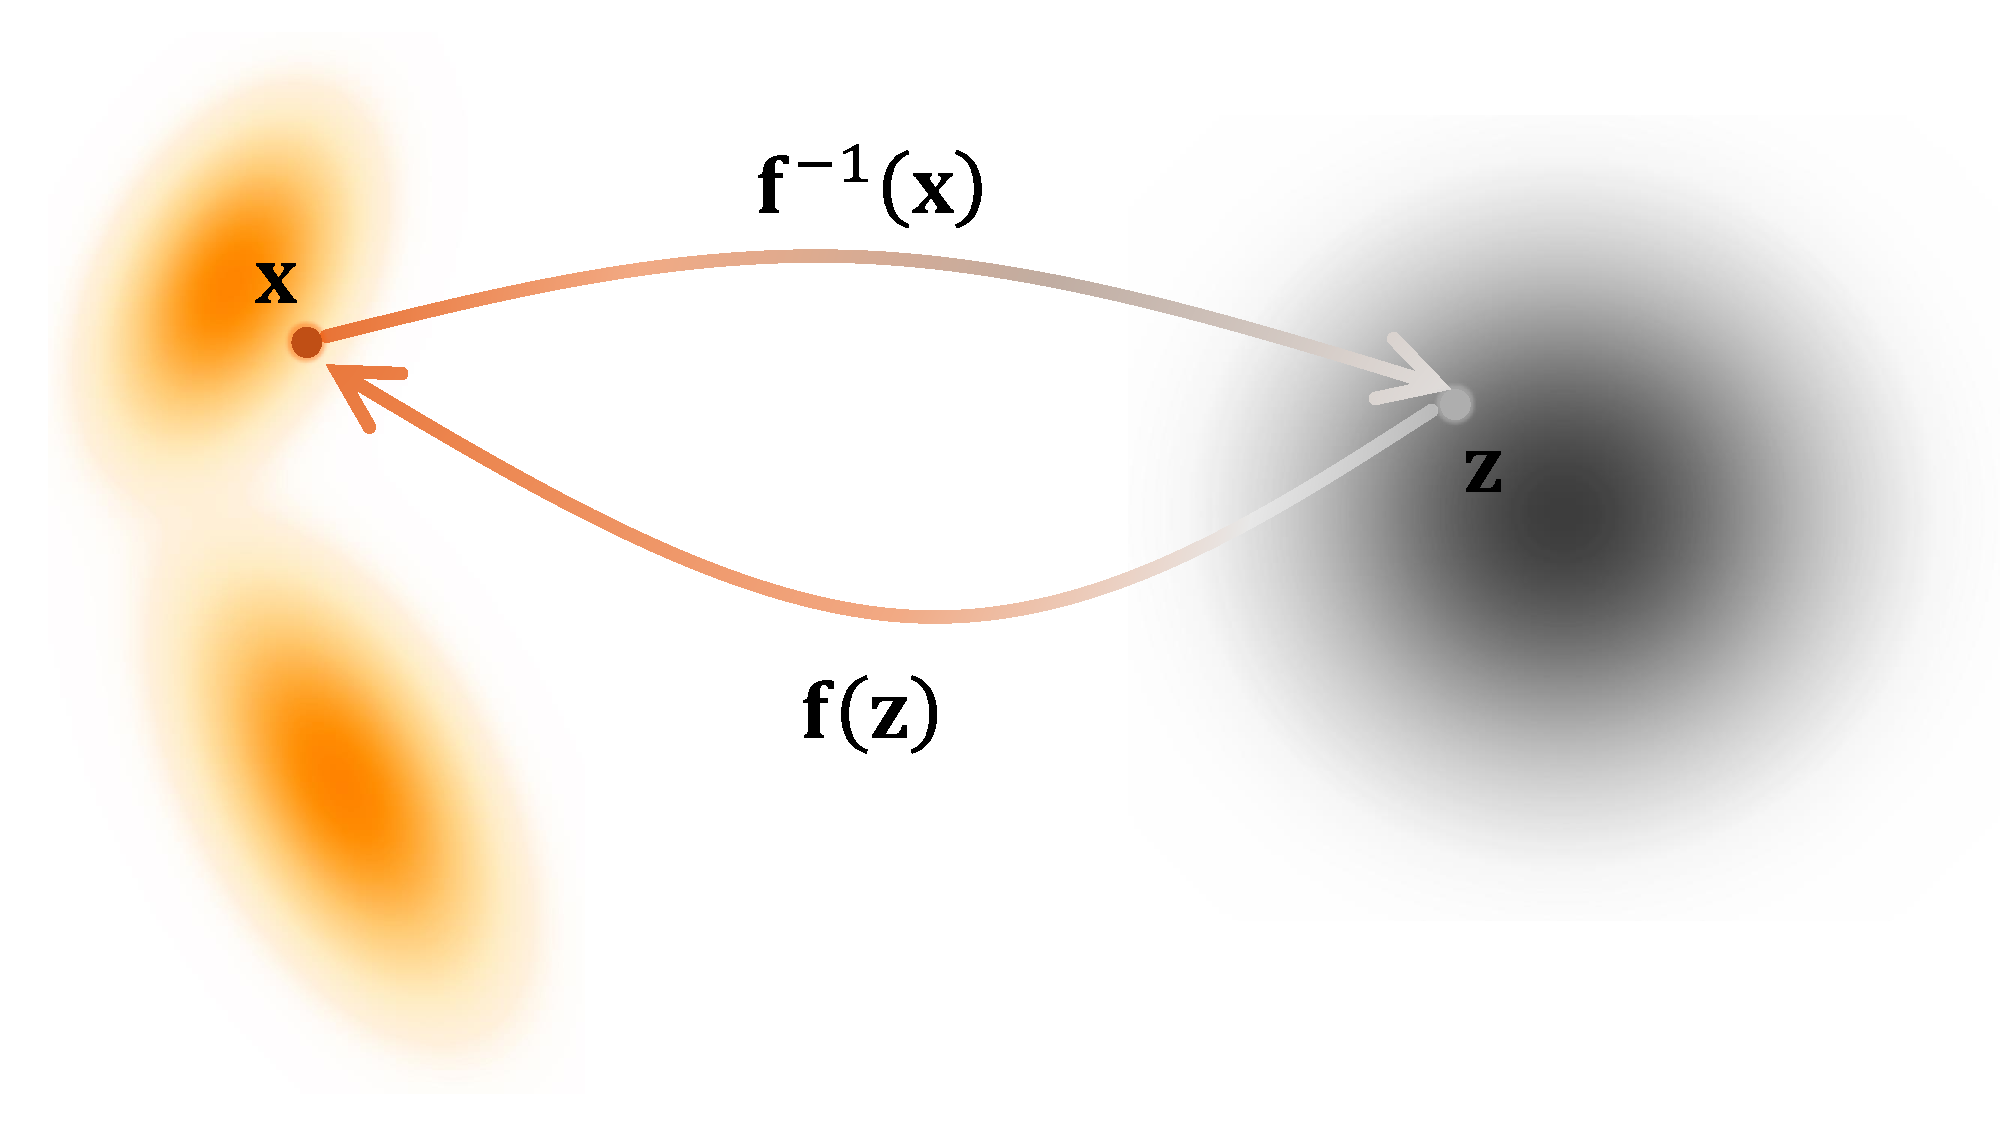
\includegraphics[width=0.76\linewidth]{Images/PartB/flow_density.pdf}
    \caption{\textbfs{可逆映射下 NF 样本移动的图示。} 它由一系列可逆函数组成 $\rvf: \rvz \mapsto \rvx$ 转换潜变量 $\rvz$ 写入数据 $\rvx$，连同逆映射 $\rvf^{-1}: \rvx \mapsto \rvz$ 重建数据。 NF 类似于编码器-解码器结构，但编码器实现为平滑可逆映射，而解码器则由其逆映射精确给出。相应的密度变化可以通过变量替换公式计算，如下所示 \Cref{eq:nf-change-of-var}. \figcredit{由作者创建。}}
    \label{fig:sample-and-change-of-variable}
\end{figure}

\subsection{归一化流}

NF~\citep{rezende2015variational} 对复杂的数据分布进行建模 $p_{\text{data}}(\rvx)$ 通过变换一个简单的先验 $p_{\text{prior}}(\rvz)$ （例如，标准高斯 $\mathcal{N}(\bm{0}, \rmI)$) 通过可逆映射
\[
\rvf_{\bm{\phi}}: \mathbb{R}^D \to \mathbb{R}^D,
\]
与 $\rvx = \rvf_{\bm{\phi}}(\rvz)$ 和 $\rvz \sim p_{\text{prior}}$。在这里， $\rvx$ 和 $\rvz$ 尺寸相同。使用变量替换公式 \Cref{eq:nf-change-of-var}，模型似然为\footnote{如果映射进一步约束为凸势的梯度，
$\rvf_\bphi = \nabla \psi_\bphi$ 与 $\psi_\bphi$ 凸，则
\Cref{eq:nf-change-of-var-log} 简化为 Monge--Ampère 关系 \Cref{eq:monge-ampere}。该偏微分方程描述了在二次成本下从一种分布到另一种分布的最优转换。参见 \Cref{ch:ot-eot} 和 \citep{huangconvex} 了解更多详情。
}
\begin{align}\label{eq:nf-change-of-var-log}
\log p_{\bm{\phi}}(\rvx) = \log p_{\text{prior}}(\rvz) + \log \left| \det \frac{\partial \rvf_{\bm{\phi}}^{-1}(\rvx)}{\partial \rvx} \right|.
\end{align}




\paragraph{训练目标。}
参数 $\bm{\phi}$ 通过最大化数据的可能性来学习：
\begin{align}\label{eq:nf-training}
\mathcal{L}_{\text{NF}}(\bm{\phi}) = \mathbb{E}_{\rvx \sim p_{\text{data}}} \left[ \log p_{\bm{\phi}}(\rvx) \right].
\end{align}
计算雅可比行列式 \Cref{eq:nf-change-of-var-log} 成本可能很高，可扩展为 $\mathcal{O}(D^3)$ 一般。

\paragraph{构造可逆变换。}






由于其雅可比行列式，单个复杂的可逆网络可能会很昂贵。相反，简单的变换（例如线性）是有效的，但缺乏表现力。为了平衡这一点，NF 采用了一系列 $L$ 可训练的可逆映射 $\{\rvf_k\}_{k=0}^{L-1}$，每个都有可有效计算的雅可比行列式：
\[
\rvf_{\bm{\phi}} = \rvf_{L-1} \circ \rvf_{L-2} \circ \cdots \circ \rvf_0.
\]
每个 $\rvf_k$ 由神经网络参数化，尽管我们省略了对 ${\bm{\phi}}$ 为了符号简单。样本变换通过
\begin{align}\label{eq:nf-seq}
\rvx_{k+1} = \rvf_k(\rvx_k), \quad k = 0, \ldots, L-1,
\end{align}
与 $\rvz=\rvx_0 \sim p_{\text{prior}}$ 和 $\rvx = \rvx_L$，对应数据。所得的（对数）密度导出为 
\begin{align}\label{eq:multi-nf-density}
\begin{aligned}
    p_{\bm{\phi}}(\rvx) &= p_{\text{prior}}(\rvx_0) \prod_{k=0}^{L-1} \left| \det \frac{\partial \rvf_k}{\partial \rvx_k} \right|^{-1}, \text{ or equivalently,}\\
\log p_{\bm{\phi}}(\rvx) &= \log p_{\text{prior}}(\rvx_0) + \sum_{k=0}^{L-1} \log \left| \det \frac{\partial \rvf_k}{\partial \rvx_k} \right|^{-1}.
\end{aligned}
\end{align}


\vspace{0.3cm}
\begin{figure}[tbh!]
    \centering
\begin{tikzpicture}[
    ->, % Sets default arrow type
    >=Stealth, % Sets default arrowhead style
    node_dist/.style={left=1.7cm of #1}, % Position nodes to the LEFT
    font=\small,
    thick
  ]

  % Define a style for the nodes
  \tikzset{state/.style={
      rectangle,
      rounded corners=3pt,
      draw=black,
      fill=gray!10,
      minimum height=35pt,
      minimum width=25pt
    }
  }

  % Place the nodes from RIGHT to LEFT
  \node[state] (x0) {$\rvx_0 $};
  \node[state] (x1) [node_dist=x0] {$\rvx_1$};
  \node[state] (x2) [node_dist=x1] {$\rvx_2$};
  \node (dots) [left=0.7cm of x2] {$\boldsymbol{\cdots}$};
  \node[state] (xL) [node_dist=dots] {$\rvx_L$};

  % Draw the arrows (edges) with labels
  
  % Top path (Generative, right to left) - Shifted up
  \path [black] ([yshift=4.5pt]x0.west)  edge node[above] {$\rvf_0$} ([yshift=4.5pt]x1.east);
  \path [black] ([yshift=4.5pt]x1.west) edge node[above] {$\rvf_1$} ([yshift=4.5pt]x2.east);
  \path [black] ([yshift=4.5pt]x2.west) edge ([yshift=4.5pt]dots.east);
  \path [black] ([yshift=4.5pt]dots.west) edge node[above, pos=0.4] {$\rvf_{L-1}$} ([yshift=4.5pt]xL.east);
  
  % Bottom path (Inference, left to right) - Shifted down
  \path ([yshift=-4.5pt]x1.east) edge node[below] {$\rvf_0^{-1}$} ([yshift=-4.5pt]x0.west);
  \path ([yshift=-4.5pt]x2.east) edge node[below] {$\rvf_1^{-1}$} ([yshift=-4.5pt]x1.west);
  \path ([yshift=-4.5pt]dots.east) edge ([yshift=-4.5pt]x2.west);
  \path ([yshift=-4.5pt]xL.east) edge node[below, pos=0.6] {$\rvf_{L-1}^{-1}$} ([yshift=-4.5pt]dots.west);

\end{tikzpicture}
\caption{\textbfs{NF 的插图。} NF 由一堆可逆映射组成
$\rvf_{\bm{\phi}} = \rvf_{L-1} \circ \rvf_{L-2} \circ \cdots \circ \rvf_0$。转换映射潜在样本 $\rvx_0 \sim p_{\mathrm{prior}}$ 数据样本 $\rvx_L \sim p_{\mathrm{data}}$. \figcredit{由作者创建。}}
    \label{fig:nf-stack}
\end{figure}\paragraph{可逆流示例。} 大量文献集中于设计单层流结构，以实现雅可比行列式的高效计算。下面，我们介绍两种具有代表性的类型：平面流~\citep{rezende2015variational}和残余流~\citep{chen2019residual,behrmann2019invertible}，后者是\Cref{subsec:NODE}发展的动力。
\subparagraph{平面流：}
平面流~\citep{rezende2015variational} 应用简单变换
\[
\rvf(\rvz)
=
\rvz
+
\rvu h(\rvw^\top\rvz+b),
\]
其中 $\rvu,\rvw\in\mathbb{R}^D$、$b\in\mathbb{R}$ 和 $h(\cdot)$ 是
激活函数。参数被适当地约束或
重新参数化以确保变换是可逆的。它的雅可比行列式
行列式具有简单的形式
\[
\left|
\det\frac{\partial\rvf(\rvz)}{\partial\rvz}
\right|
=
\left|
1+h'(\rvw^\top\rvz+b)\,\rvw^\top\rvu
\right|,
\]
使变量变化计算变得高效。

\subparagraph{剩余流：}
将变换 $\rvf$ 定义为
\begin{align}\label{eq:residual-flow}
\rvf(\rvz) = \rvz + \rvv(\rvz),
\end{align}
与 $\rvv$ 收缩（Lipschitz 常数 $< 1$）。这通过巴纳赫不动点定理确保了可逆性。

雅可比行列式的对数行列式简化为迹展开式：
\begin{align}\label{eq:log-det-tr}
    \log \Bigg|\det \frac{\partial \rvf(\rvz)}{\partial \rvz} \Bigg| &= \log \left( \det \frac{\partial \rvf(\rvz)}{\partial \rvz} \right) \nonumber\\
    &= \Tr\left(\log\left(\frac{\partial \rvf(\rvz)}{\partial \rvz}\right)\right) \nonumber\\
    &= \Tr\left(\log\left(\rmI + \frac{\partial \rvv(\rvz)}{\partial \rvz}\right)\right) \nonumber\\
    &= \sum_{k=1}^{\infty} \frac{(-1)^{k+1}}{k} \Tr\left(\left(\frac{\partial \rvv(\rvz)}{\partial \rvz}\right)^k\right),
\end{align}
通过跟踪估计器~\citep{hutchinson1989stochastic} 提高评估效率。

\paragraph{采样与推理.}
从 NF 中采样非常简单：绘制 $\rvx_0 \sim p_{\text{prior}}$ 并计算 $\rvx = \rvf_{\bm{\phi}}(\rvx_0)$。确切的可能性从 \Cref{eq:multi-nf-density} 获得。


\subsection{神经常微分方程}\label{subsec:NODE}
\begin{figure}[th!]
    \centering
    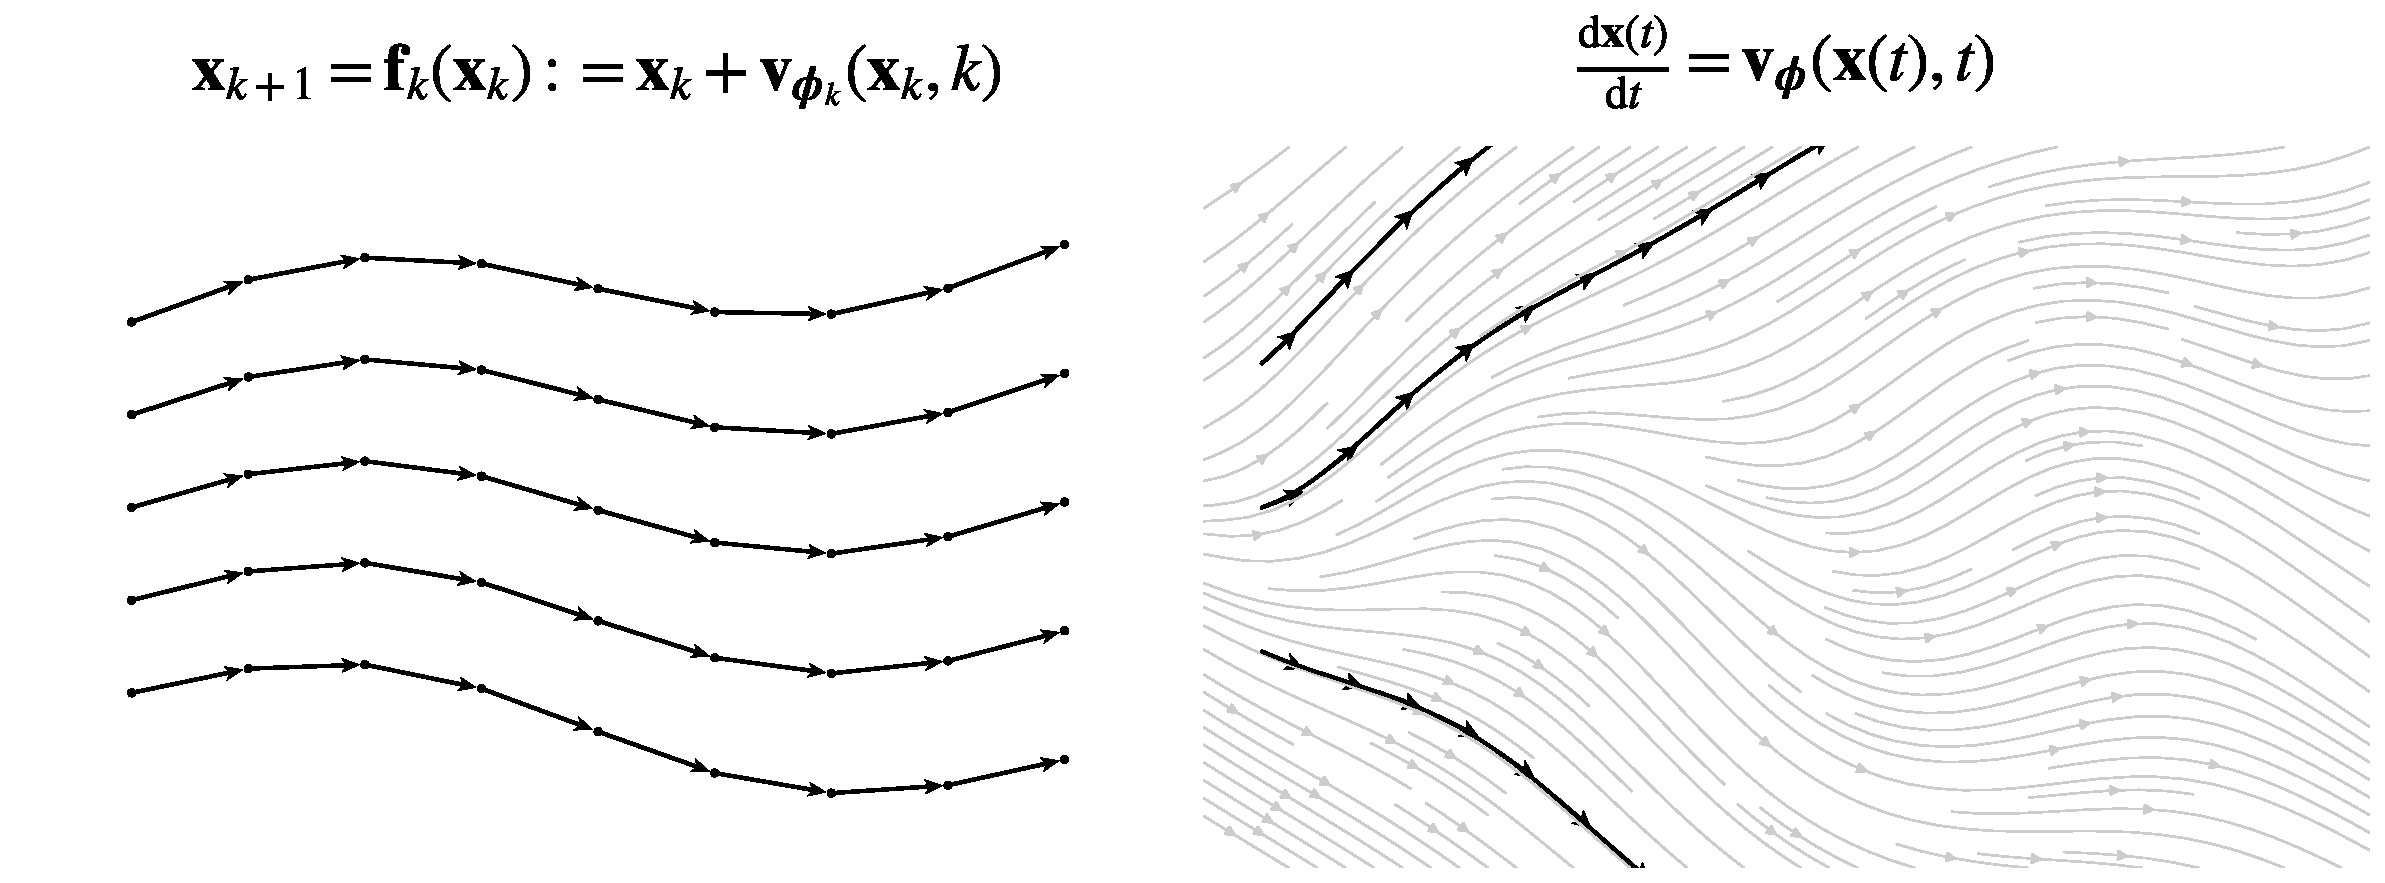
\includegraphics[width=\linewidth]{Images/PartB/discrete_vs_continuous_side_by_side_white.pdf}
    \caption{\textbfs{离散-与连续时间归一化流。}（左）离散 NF 通过可逆映射 $\mathbf{x}_{k+1} = \mathbf{f}_k(\mathbf{x}_k)$ 的有限序列传输样本，
产生逐步的、非交叉的轨迹（带箭头的点）。 （右）连续 NF（神经常微分方程）沿着 $\frac{\diff\mathbf{x}(t)}{\diff t} = \mathbf{v}_{\boldsymbol{\phi}}(\mathbf{x}(t),t)$ 的积分曲线演化状态，
其中带有切线箭头的黑色路径显示在灰色矢量场上。 \figcredit{由作者创建。}}
    \label{fig:nf-cnf}
\end{figure}
















\paragraph{从离散时间 NF 到连续时间 NF（神经常微分方程）.}
离散 NF 通过 $L$ 可逆组件传输样本
映射。为了获得有意义的连续深度限制，我们编写每一层
作为一个小的剩余更新：
\[
\rvx_{k+1}
=
\rvx_k+\Delta t\,\rvv_{\bm{\phi}}(\rvx_k,t_k),
\qquad
t_k=k\Delta t,
\qquad
\Delta t=\frac{T}{L}.
\]
这里，$\rvv_{\bm{\phi}}$指定每个点的方向
移动，而$\Delta t$控制一层的大小。

该极限的几何意义如图所示
\Cref{fig:bijection-continuity}。随着$L$的增加，同样
源到目标的传输被分为更接近同一的双射。
样本轨迹被更精细地解析，并且变形
周围的参考网格变得逐渐平滑。

如$L\rightarrow\infty$和$\Delta t\rightarrow 0$，离散层
指数变为连续时间，产生 ODE
\[
\frac{\diff \rvx(t)}{\diff t}
=
\rvv_{\bm{\phi}}(\rvx(t),t).
\]
这种连续深度模型称为神经 ODE 或连续
归一化流。\begin{figure}[th!]
    \centering
    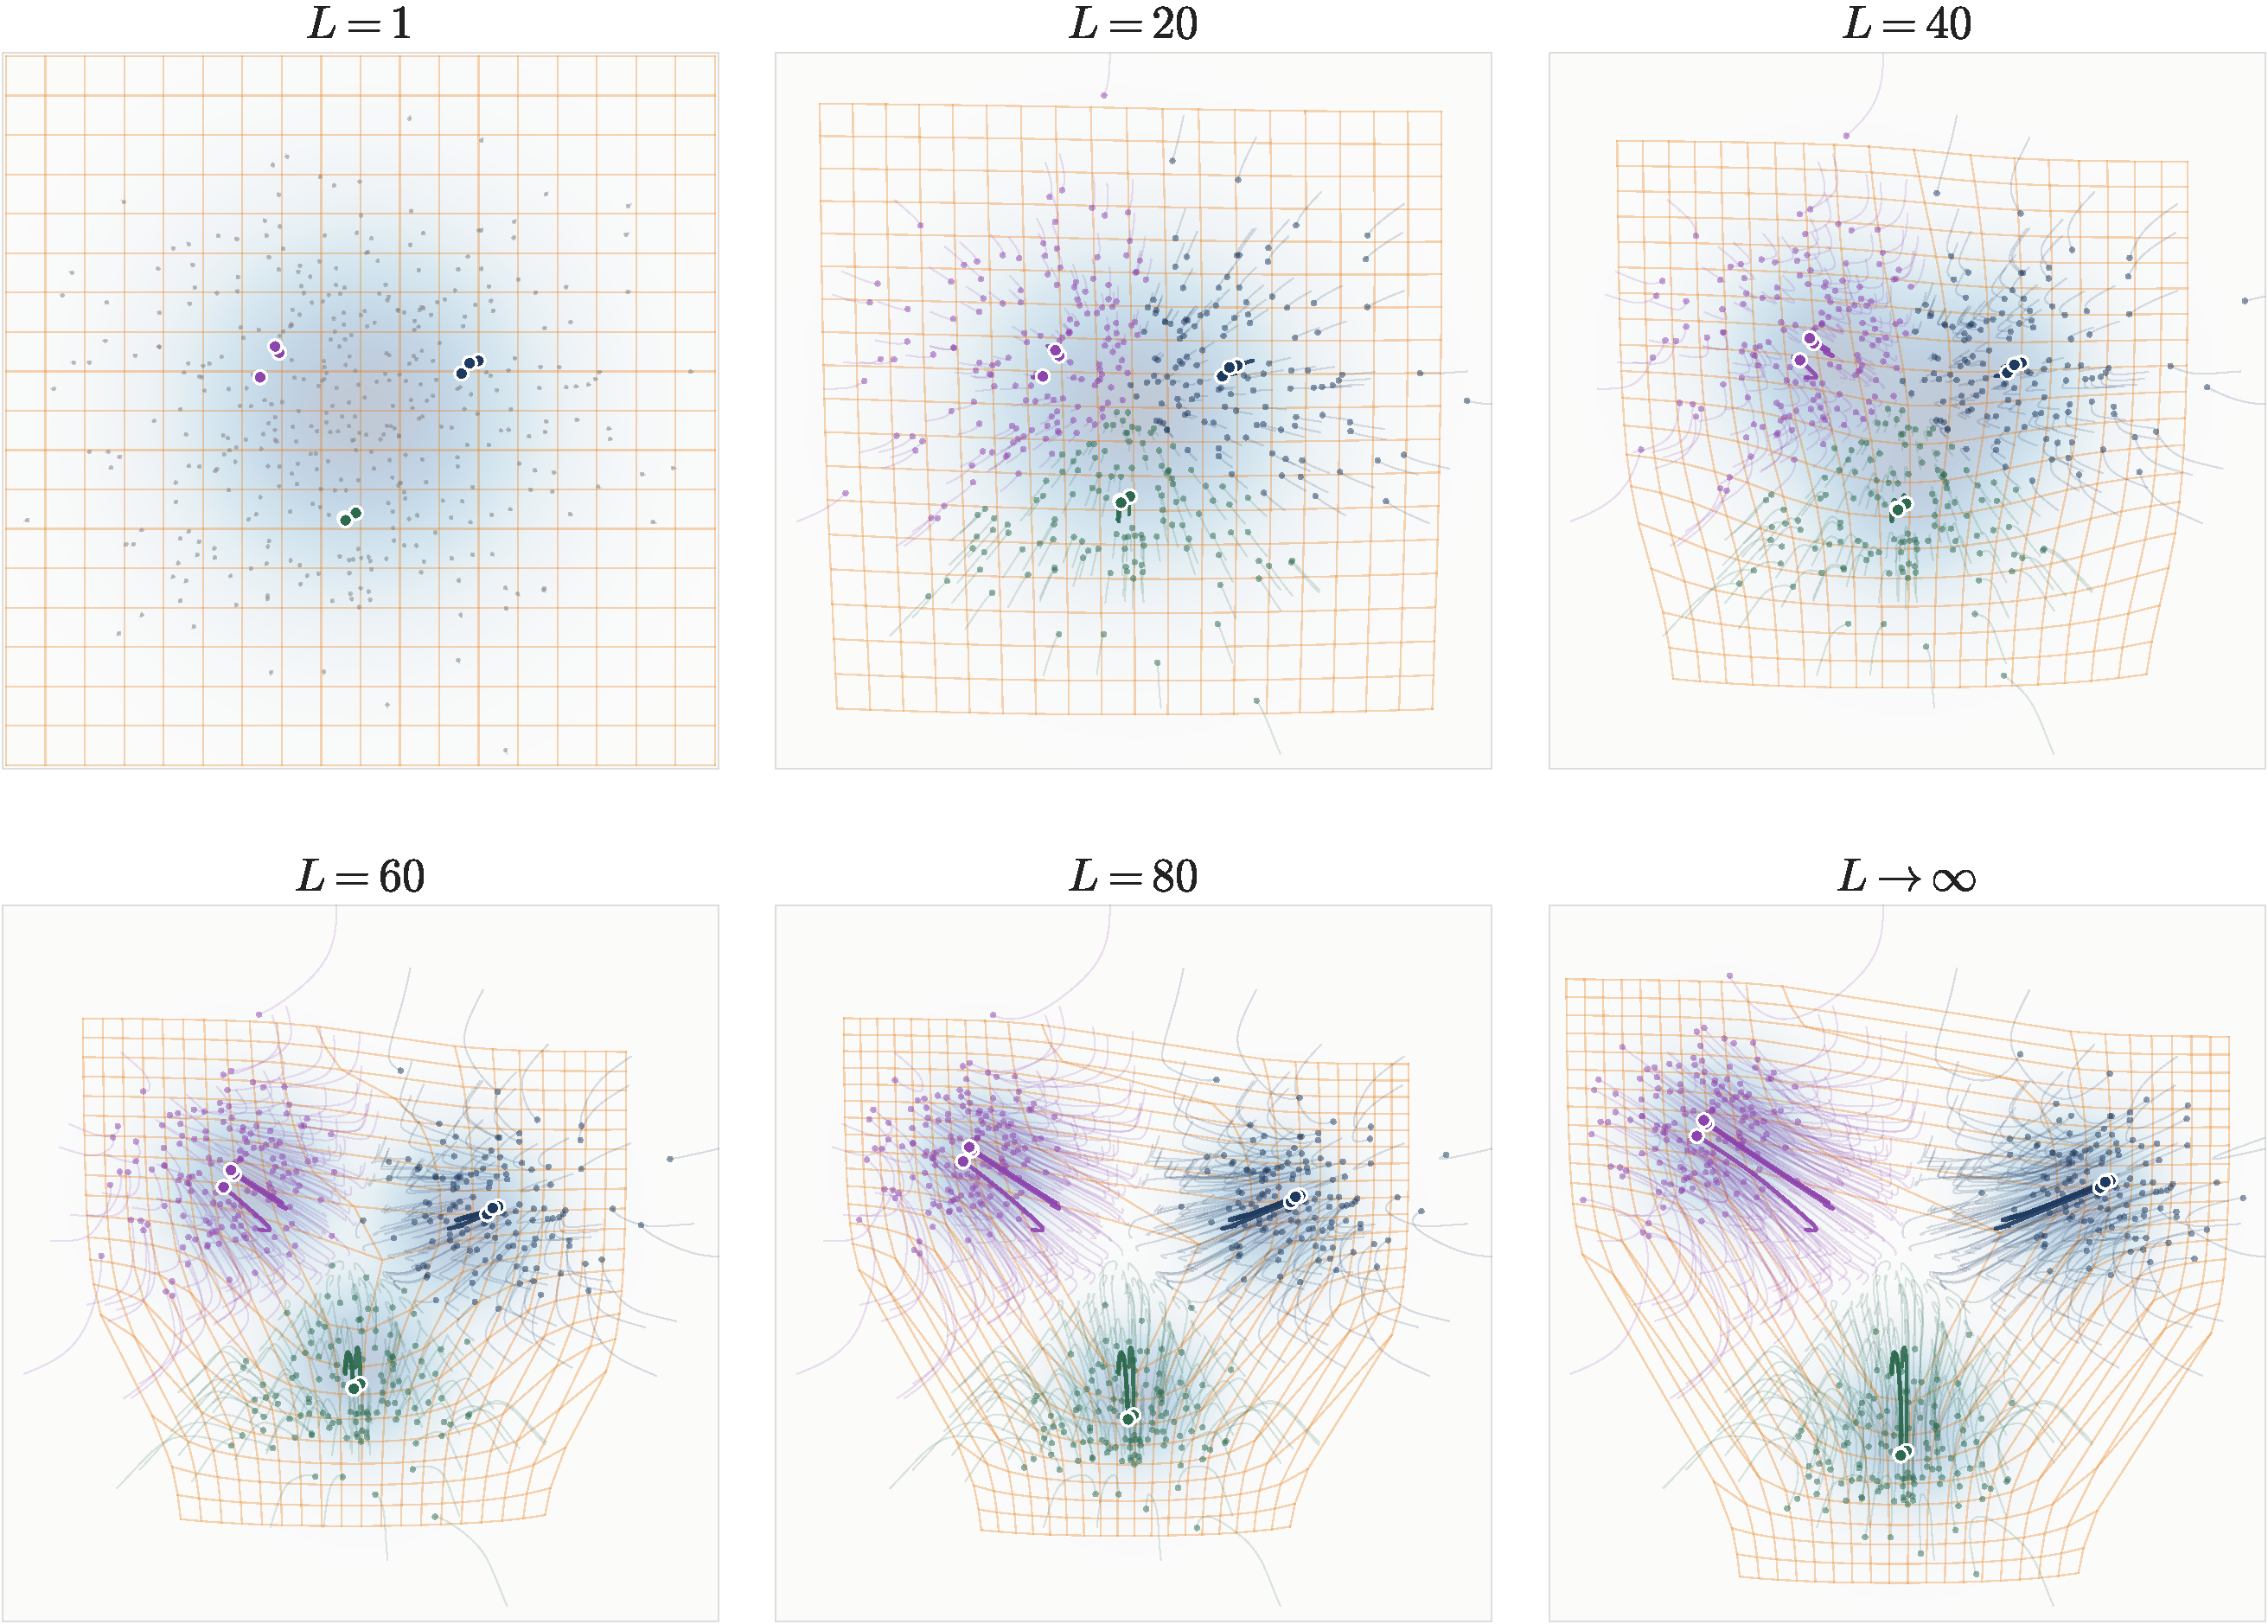
\includegraphics[width=\linewidth]{Images/PartB/cov_2d_layers.pdf}
    \caption{\textbfs{从离散双射到连续传输流。}
    每个面板都显示了通过组合 $L$ 可逆层构建的传输。
    从源分布（高斯）开始，各层逐渐移动
    彩色样本朝向具有三种模式的目标分布。的
    橙色参考网格显示周围空间在过程中如何变形
    这种运输。只有几层，每层都相对
    大而离散的变化。随着$L$的增加，运输被划分
    分成更多、更小的更新，因此样本轨迹和网格
    变形变得更加平滑。如果总运输时间 $T$ 固定
    每层的步长为 $\Delta t=T/L$，则：
    $L\rightarrow\infty$，堆叠双射接近连续
    时间相关的流。传输密度根据
    \Cref{eq:continuity_eq} 中的连续性方程。
    \figcredit{由作者使用AI辅助编码创建。}}
    \label{fig:bijection-continuity}
\end{figure}


\paragraph{ 神经常微分方程的形式化设置.}
神经常微分方程通过以下方式定义连续变换：
\begin{align}\label{eq:neural-ode}
    \frac{\diff \rvx(t)}{\diff t} = \rvv_{\bm{\phi}}(\rvx(t), t),\quad t\in [0,T]
\end{align}
其中：
\begin{itemize}
    \item $ \rvx(t) \in \mathbb{R}^D $ 为 $t$ 时刻的状态；为了简洁起见，我们有时会写成 $\rvx_t$；
    \item $\rvv_{\bm{\phi}}(\rvx(t), t)$ 是由 $\bm{\phi}$ 参数化的神经网络。
\end{itemize}


\subparagraph{NODE.}目标
从初始条件 $\rvx(0) \sim p_{\text{prior}}$ 开始，ODE 随着时间的推移不断演化状态，引入一系列边缘分布 $p_{\bm{\phi}}(\rvx_t, t)$（类似于 PF-ODE！）\footnote{我们采用翻转时间约定，其中 $t = 0$ 表示先验（源），$t = 1$ 表示数据（目标）分布。先验可互换地写为 $p_{\bm{\phi}}(\rvx(0), 0)$、$p_{\text{prior}}(\rvx(0), 0)$ 或简称为 $p_{\text{prior}}(\rvz)$。
}。 

目标是学习神经向量场 $\rvv_{\bm{\phi}}$，它直观地表示沿着数据空间中的连续轨迹传输点的速度。通过学习该速度，$t=T$ 处的终端分布与目标分布 $p_{\mathrm{data}}(\cdot)$ 相匹配。这种连续变换将离散归一化流和神经常微分方程统一在一个框架内。



\paragraph{连续时间变量替换公式.}
类似于 \Cref{eq:nf-change-of-var} 或 \Cref{eq:multi-nf-density}，
\citet{chen2018neural} 导出了连续时间模拟
变量替换公式。对于随时间变化的密度
$p_{\bm{\phi}}(\rvx(t),t)$ 下演变的进程 $\rvx(t)$
\Cref{eq:neural-ode}，即所谓\emph{瞬时
变量替换公式}为
\[
\frac{\diff}{\diff t}
\log p_{\bm{\phi}}(\rvx(t),t)
=
-\nabla_{\rvx}\cdot
\rvv_{\bm{\phi}}(\rvx(t),t).
\]
此处，沿 ODE 轨迹 $\rvx(t)$ 求导。

因此，如果 $\rvx(0)\sim p_{\mathrm{prior}}$ 和 ODE 传输
在从 $t=0$ 到 $t=T$ 之前，集成此恒等式给出
\begin{align}\label{eq:NODE-likelihood}
\log p_{\bm{\phi}}(\rvx(T),T)
=
\log p_{\mathrm{prior}}(\rvx(0))
-
\int_0^T
\nabla_{\rvx}\cdot
\rvv_{\bm{\phi}}(\rvx(t),t)
\,\diff t.
\end{align}
该表达式通过数值积分提供似然评估，
这反过来又可以实现模型的最大似然训练。

虽然这个公式乍一看可能有些陌生，但它与福克-普朗克方程密切相关。特别地，它可以理解为沿轨迹的形式 \emph{连续性方程}，这是福克-普朗克方程的确定性零扩散情况（参见 \Cref{app:continuity}）。它也可以解释为离散变量替换公式的连续时间极限
\Cref{eq:multi-nf-density}。我们将结果总结如下。

\lemp{变量瞬时变化}{instant-change-of-var}{
让 $\rvz(t)$ 是一个具有时间依赖性密度的连续随机过程
$p(\rvz(t),t)$，并假设它根据 ODE 演化
\begin{align*}
\frac{\diff\rvz(t)}{\diff t}
=
\mathbf{F}(\rvz(t),t).
\end{align*}
假设有足够的规律性，以便很好地定义 ODE 流和演化密度，则沿轨迹的对数密度满足
\begin{align}\label{eq:instant-change-of-var}
\frac{\diff}{\diff t}
\log p(\rvz(t),t)
=
-\nabla_{\rvz}\cdot
\mathbf{F}(\rvz(t),t).
\end{align}
}{
这是根据连续性方程和链式法则得出的。我们在中提出了详细的替代推导 \Cref{app-sec:flow-proof}.}


\subparagraph{与离散时间公式的连接。}  
节点可能性 \Cref{eq:NODE-likelihood},
\[
\log p_{\bm{\phi}}(\rvx(T), T) = \log p_{\text{prior}}(\rvx(0), 0) - \int_0^T \nabla_\rvx \cdot \rvv_{\bm{\phi}}(\rvx(t), t) \diff t,
\]
可以看作是离散归一化流公式的连续时间模拟 \Cref{eq:multi-nf-density}:
\[
\log p_{\bm{\phi}}(\rvx_L) = \log p_{\text{prior}}(\rvx_0) - \sum_{k=0}^{L-1} \log \left| \det \frac{\partial \rvf_k}{\partial \rvx_k} \right|.
\]
积分反映了求和，并且迹运算符取代了对数行列式，如中讨论的 \Cref{eq:log-det-tr}。这些相似之处在引理的证明中得到了进一步探讨。

\paragraph{训练节点。}  
基于 \Cref{eq:NODE-likelihood}，节点学习参数化速度场 $\rvv_{\bm{\phi}}$ 这样的终端分配
\[
p_{\bm{\phi}}(\cdot, T) \approx p_{\text{data}},
\]
轨迹从潜变量演变而来 $\rvx(0) \sim p_{\text{prior}}$ 通过 ODE 流程。训练遵循 MLE 框架 \Cref{eq:MLE}:
\[
\mathcal{L}_{\text{NODE}}(\bm{\phi}) := \mathbb{E}_{\rvx \sim p_{\text{data}}} \big[\log p_{\bm{\phi}}(\rvx, T)\big].
\]

\subparagraph{精确的对数似然计算。} 
计算 $\log p_{\bm{\phi}}(\mathbf{x}, T)$ 用于数据点 $\mathbf{x}$，我们对变量替换公式进行积分 \eqref{eq:NODE-likelihood}:
\begin{align}
\log p_{\bm{\phi}}(\mathbf{x}, T) = \log p_{\text{prior}}(\mathbf{z}(0)) - \int_0^T \nabla_{\mathbf{z}} \cdot \mathbf{v}_{\bm{\phi}}(\mathbf{z}(t), t) \diff t.
\end{align}
在这里， $\mathbf{z}(t)$ 逆向求解 ODE $t = T$ 至 $t = 0$:
\[
\frac{\diff\mathbf{z}(t)}{\diff t} = \mathbf{v}_{\bm{\phi}}(\mathbf{z}(t), t)
\]
与 $\mathbf{z}(T) = \mathbf{x}$。前一术语 $\log p_{\text{prior}}(\mathbf{z}(0))$ 易于处理标准发行版。这使得神经常微分方程中能够进行精确的基于似然的训练和评估。

\subparagraph{基于梯度的优化。}  
最大化 $\mathcal{L}_{\text{NODE}}$ 需要通过 ODE 求解器进行反向传播。伴随灵敏度法~\citep{pontryagin2018mathematical, chen2018neural} 通过辅助 ODE 计算梯度 $\mathcal{O}(1)$ 内存复杂性，但由于每一步的数值积分，NODE 训练仍然很昂贵。

\paragraph{使用节点进行推理。}  
使用经过训练的模型进行采样 $\rvv_{\bm{\phi}^\times}$ 通过绘图获得收益 $\rvx(0) \sim p_{\text{prior}}$ 并向前积分（通过数值求解器）：
\[
\rvx(T) = \rvx(0) + \int_0^T \rvv_{\bm{\phi}^\times}(\rvx(t), t)   \diff t.
\]
终端状态 $\rvx(T)$ 近似样本 $p_{\text{data}}$.此外，我们注意到对于任何向量场 $\rmF$，以下恒等式成立：
\[
    \Tr\left(\frac{\partial \rmF}{\partial \rvz(t)} \right) = \nabla_{\rvz} \cdot \rmF.
\]
因此，可以使用随机迹有效地估计散度
估计器，例如 Hutchinson 估计器~\citep{hutchinson1989stochastic}，
无需明确构建完整的雅可比行列式。这使得可能性
评估在高维环境中更加实用。然而，因为
然后从随机样本中估计轨迹，得到的数值
对数似然估计是随机的，而不是对
分歧。

在\Cref{fig:bijection-continuity}中看到了多少个小双射
接近连续传输流，我们现在问一个实际问题：
\begin{question}
    我们如何在不重复求解常微分方程的情况下了解其速度场
训练期间？
\end{question}
 这个问题很自然地引出了流匹配，即
通过免模拟回归直接学习速度场
目标并提供扩散模型的基于流的视角。




























\newpage
\clearpage
\section{\texorpdfstring{流匹配框架}{流匹配框架}}\label{sec:flow-matching-framework}

两者均分数 SDE~(\Cref{ch:score-sde}) 和
NODEs~(\Cref{sec:flow-based-method}) 将生成建模描述为
连续运输过程。 Score SDE 通过以下方式制定此传输
随机动力学以及相关的 PF-ODE，
而节点直接参数化确定性 ODE。在标准中
生成设置，两者都旨在传输简单的高斯先验
$p_{\mathrm{prior}}$ 进入数据分布$p_{\mathrm{data}}$。

NODE 的一个实际限制是基于似然的训练需要
反复求解 ODE。 \emph{流匹配}（FM）
Framework~\citep{lipman2022flow,lipman2024flow,tongimproving} 避免了这种情况
通过训练神经网络直接预测速度场来计算成本
通过回归目标。因此需要 ODE 积分
生成，但不在训练循环内，进行 FM 训练
免模拟。

更一般地说，FM 不限于高斯到数据的传输。它
考虑源分布 $p_{\mathrm{src}}$ 和目标
分布 $p_{\mathrm{tgt}}$，两者都假设很容易从中采样。
标准生成模型被恢复为特殊情况
\[
p_{\mathrm{src}}=p_{\mathrm{prior}},
\qquad
p_{\mathrm{tgt}}=p_{\mathrm{data}},
\]
其中 $p_{\mathrm{prior}}$ 是典型的高斯分布。

本节我们采用FM观点\footnote{几种相关方法共享使用连续时间流在端点分布之间传输的核心思想，尽管它们的表述略有不同。其中包括流匹配 (FM)~\citep{lipman2022flow,neklyudov2023action}，整流流 (RF)~\citep{liu2022rectified,heitz2023iterative}和随机插值~\citep{albergo2023stochastic,albergobuilding,ma2024sit}。在这里，我们使用 FM 作为统一术语。}
其目标是学习与时间相关的速度场
$\mathbf{v}_t(\rvx_t)$ 其关联的 ODE 沿着规定的概率路径传输样本 $\{p_t\}_{t\in[0,1]}$ 满意
\[
p_0=p_{\mathrm{src}},
\qquad
p_1=p_{\mathrm{tgt}}.
\]
当 $p_{\mathrm{src}}$ 是高斯分布，我们将此设置称为
\emph{高斯流匹配}。因此，FM 既提供了用于生成建模的免模拟训练方法，又提供了用于学习任意端点分布之间的连续传输的通用框架。












































\subsection{基于分数的方法的教训}\label{subsec:lesson-score}

我们重新审视 Score SDE 框架（\Cref{ch:score-sde}) 使用略有不同但等效的公式来提取激发 FM 方法的关键见解。该分析揭示了扩散模型如何隐式学习概率流并激发更直接的表述。


\paragraph{步骤 1：定义条件路径及其边缘密度。}

\begin{figure}[th!]
    \centering
    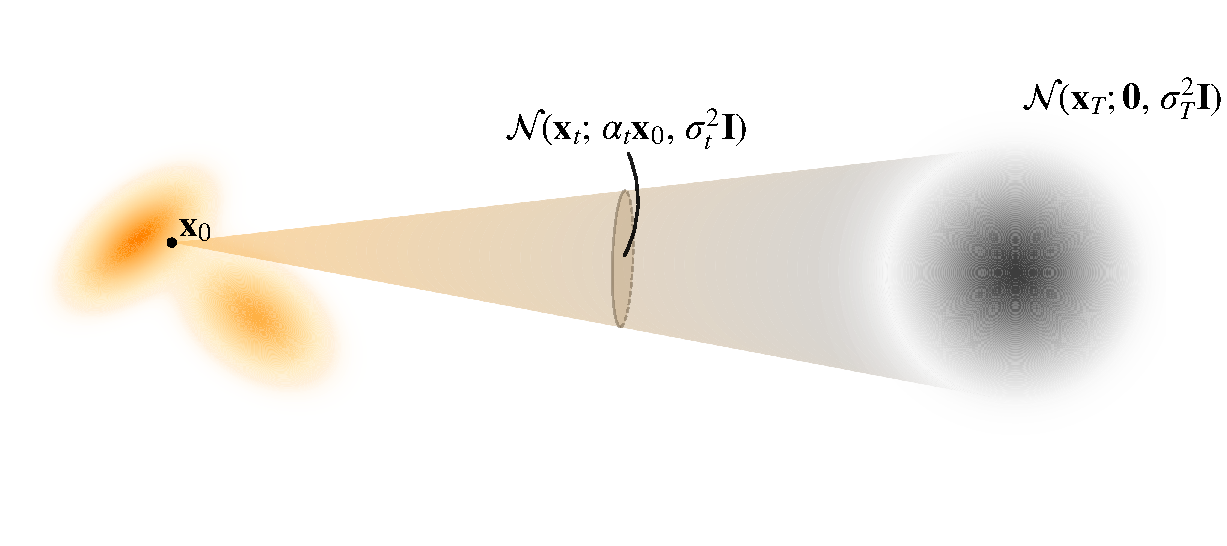
\includegraphics[width=\linewidth]{Images/PartB/data_vs_prior_cone_with_oval.pdf}
    
    \caption{\textbfs{条件转换分布的图示。} 
$p_t(\rvx_t | \rvx_0) = \mathcal{N}(\rvx_t;\alpha_t \rvx_0,\sigma_t^2 \mathbf{I})$，定义数据样本的（高斯）条件概率路径 
$\rvx_0 \sim p_{\text{data}}$ （左）朝向高斯先验 
$p_{\text{prior}}$ （右）。 \figcredit{由作者创建。}}
    \label{fig:data-prior-conditioning}
\end{figure}

扩散模型指定连续时间密度族 $\{p_t\}_{t \in [0,1]}$ 传输一个简单的先验 $p_{\text{prior}}$ （例如，高斯）在 $t=1$，用作源，到目标数据分布 $p_{\text{data}}$ 在 $t=0$:
\[
p_1(\rvx_1) = p_{\text{prior}}(\rvx_1), \quad p_0(\rvx_0) = p_{\text{data}}(\rvx_0).
\]
该路径是通过前向条件分布隐式定义的
\begin{align}\label{eq:lesson-dm-conditional-path}
    p_t(\rvx_t|\rvx_0) = \mathcal{N}(\rvx_t; \alpha_t \rvx_0, \sigma_t^2 \mathbf{I}), \quad \rvx_0\sim p_{\text{data}}
\end{align}
产生边缘密度
\[
p_t(\rvx_t) := \int p_t(\rvx_t |\rvx_0)  p_{\text{data}}(\rvx_0) \mathrm{d}\rvx_0.
\]
方差增加 $\sigma_t^2$ 条件高斯驱动演化 $p_t$ 朝向高斯先验。

\paragraph{第 2 步：速度场。}
边缘密度的时间演化 $p_t$ 由速度场控制 $\rvv_t : \mathbb{R}^D \to \mathbb{R}^D$，由 Fokker-Planck 方程导出：
\begin{align}\label{eq:dm-velocity}
    \rvv_t(\rvx) := f(t)\rvx - \frac{1}{2}g^2(t)\nabla_{\rvx} \log p_t(\rvx),
\end{align}
定义通过 PF-ODE 的确定性粒子流：
\[
\frac{\diff \rvx(t)}{\diff t} = \underbrace{f(t)\rvx(t) - \frac{1}{2}g^2(t)\nabla_{\rvx} \log p_t\big(\rvx(t)\big)}_{\rvv_t(\rvx(t))}.
\]
此 ODE 传输初始随机变量 $\rvx(0) \sim p_{\text{data}}$ 及时转发或 $\rvx(1) \sim p_{\text{prior}}$ 时间上落后，使得边缘密度的演变 $\rvx(t)$ 匹配 $p_t$ 每次 $t \in [0,1]$  （请参阅下面的“基本规则”）。标量函数 $f(t)$ 和 $g(t)$ 由相关前向 SDE 的系数或等效的高斯核参数确定 $\alpha_t$ 和 $\sigma_t$ 在条件路径中定义（参见引理~\ref{forward-sde}).


\paragraph{第 3 步：通过条件策略学习。}
PF-ODE 速度 \Cref{eq:dm-velocity} 取决于边缘分数
$\nabla_{\rvx_t}\log p_t(\rvx_t)$，一般不为人所知。因此，基于分数的方法使用神经网络来学习该分数
$\rvs_{\bm{\phi}}(\rvx_t,t)$ 通过理想的分数匹配目标
\[
\mathcal{L}_{\text{SM}}(\bm{\phi})
=
\mathbb{E}_{t\sim\mathcal{U}[0,1],\,\rvx_t\sim p_t}
\left[
\left\|
\rvs_{\bm{\phi}}(\rvx_t,t)
-
\nabla_{\rvx_t}\log p_t(\rvx_t)
\right\|^2
\right].
\]
一旦了解了分数，就可以从中获得 PF-ODE 速度：
\[
\rvv_t(\rvx_t)
=
f(t)\rvx_t
-
\frac{1}{2}g^2(t)
\nabla_{\rvx_t}\log p_t(\rvx_t),
\]
与 $\rvs_{\bm{\phi}^\times}(\rvx,t) \approx \nabla_{\rvx_t}\log p_t(\rvx)$

困难在于计算回归目标时边缘分数本身是不可访问的。如在 \Cref{ch:score-based}我们使用调节技巧克服了这个问题。条件分布 $p_t(\rvx_t|\rvx_0)$ 易于处理，其条件分数满足
\begin{align}\label{eq:marginal-oracle-score}
\nabla_{\rvx_t}\log p_t(\rvx_t)
=
\mathbb{E}_{\rvx_0\sim p(\cdot|\rvx_t)}
\left[
\nabla_{\rvx_t}\log p_t(\rvx_t|\rvx_0)
\right].
\end{align}
这激发了去噪分数匹配目标
\[
\mathcal{L}_{\text{DSM}}(\bm{\phi})
:=
\mathbb{E}_{t,\,\rvx_0\sim p_{\mathrm{data}},\,
\rvx_t\sim p_t(\cdot|\rvx_0)}
\left[
\left\|
\rvs_{\bm{\phi}}(\rvx_t,t)
-
\nabla_{\rvx_t}\log p_t(\rvx_t|\rvx_0)
\right\|^2
\right].
\]
如定理所示~\ref{thm:sm-dsm}, $\mathcal{L}_{\text{SM}}$ 和
$\mathcal{L}_{\text{DSM}}$ 仅相差一个独立的常数
$\bm{\phi}$ 因此具有相同的总体最小化：
\[
\rvs^*(\rvx_t,t)
=
\mathbb{E}_{\rvx_0\sim p(\cdot|\rvx_t)}
\left[
\nabla_{\rvx_t}\log p_t(\rvx_t|\rvx_0)
\right]
=
\nabla_{\rvx_t}\log p_t(\rvx_t).
\]

重要的是，相同的调节原理也可以直接在 PF-ODE 速度级别上表达。定义条件速度
\[
\rvv_t(\rvx_t|\rvx_0)
:=
f(t)\rvx_t
-
\frac{1}{2}g^2(t)
\nabla_{\rvx_t}\log p_t(\rvx_t|\rvx_0).
\]
使用 \Cref{eq:marginal-oracle-score}，我们立即得到
\[
\rvv_t(\rvx_t)
=
\mathbb{E}_{\rvx_0\sim p(\cdot|\rvx_t)}
\left[
\rvv_t(\rvx_t|\rvx_0)
\right].
\]
因此，基于分数的扩散通过易处理的条件目标学习分数，然后用它来构造 PF-ODE 速度。流匹配将相同的条件到边缘原理直接应用于速度场。
\begin{figure}
    \centering
    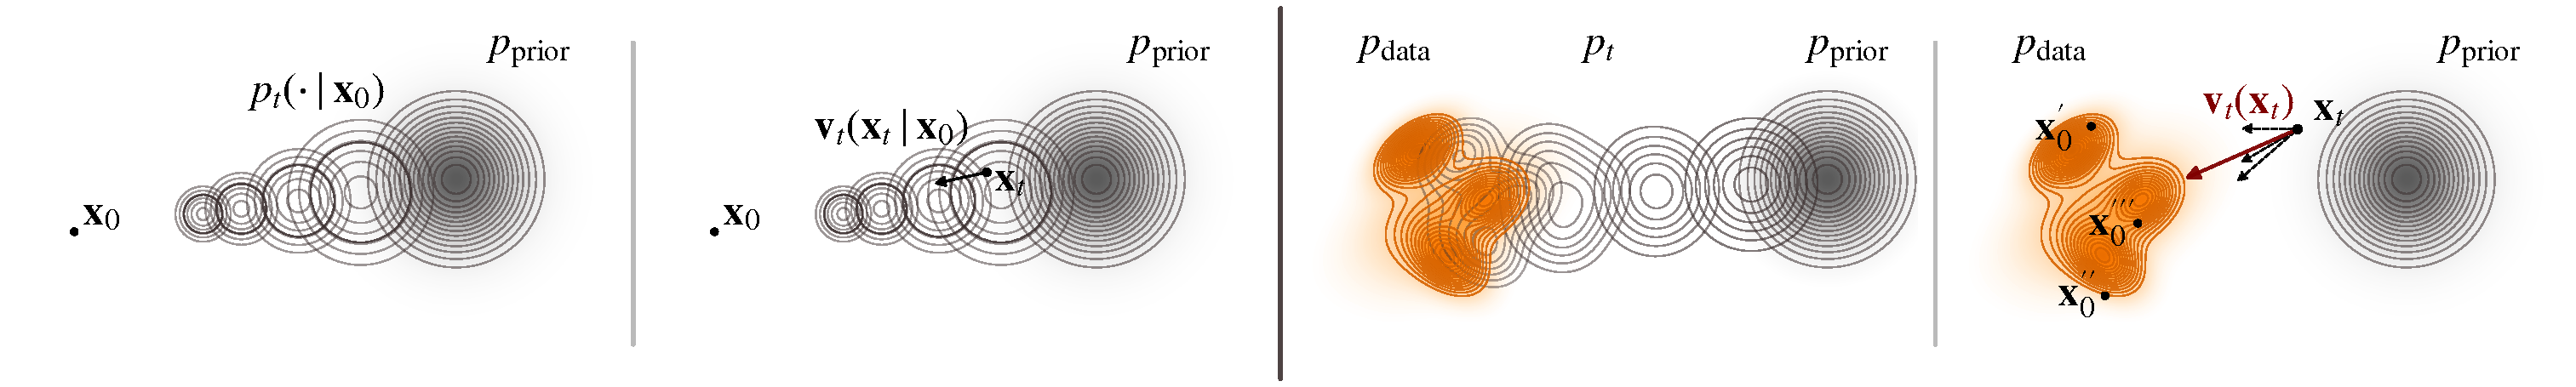
\includegraphics[width=\linewidth]{Images/PartB/four_panel_simple.pdf}
    \caption{\textbfs{扩散中条件视角与边缘视角的图示。} （这个数字的动机是 \citet{lipman2024flow}.) (1) 条件高斯路径 $p_t(\cdot|\mathbf{x}_0)$，显示从固定密度扩展的密度 $\mathbf{x}_0$ 朝前。 (2) 条件速度 $\mathbf{v}_t(\mathbf{x}_t|\mathbf{x}_0)=f(t)\rvx_t - \tfrac{1}{2}g^2(t) \nabla_{\rvx_t} \log p_t(\rvx_t|\rvx_0)$。 (3) 边缘密度 $p_t$，传输数据分布 $p_{\mathrm{data}}$ （橙色）进入之前 $p_{\mathrm{prior}}$ （灰色）。 (4) 边缘速度 $\mathbf{v}_t(\mathbf{x}_t)=f(t)\rvx_t - \tfrac{1}{2}g^2(t) \nabla_{\rvx_t} \log p_t(\rvx_t)$，通过对条件方向求平均值获得 $\mathbf{x}_t$ 到多个可能的起源（虚线），产生红色箭头。在具有单侧调节的 FM 框架中 $\rvz=\rvx_0$，同图适用于 $\rvv_t(\rvx_t|\rvx_0)$ 和 $\rvv_t(\rvx_t)$，无需明确以分数形式书写 
$\nabla_{\rvx_t}\log p_t(\rvx_t|\rvx_0)$ 或 $\nabla_{\rvx_t}\log p_t(\rvx_t)$.
\figcredit{由作者创建。}}
    \label{fig:conditional-marginal}
\end{figure}

\paragraph{基本规则：福克-普朗克方程。}
边缘密度 $p_t$ 根据福克-普朗克方程演化：
\begin{mdframed}
\begin{align*}
    \frac{\partial p_t(\rvx)}{\partial t} + \nabla \cdot \Bigg( \underbrace{\left(f(t)\rvx - \frac{1}{2}g^2(t) \nabla_\rvx \log p_t(\rvx)\right)}_{\rvv_t(\rvx)}  p_t(\rvx) \Bigg) = 0.
\end{align*}
\end{mdframed}
该偏微分方程确保 PF-ODE 给出的密度与前向 SDE 的边缘分布相匹配。要看到这一点，请回忆一下 \emph{流映射} $\bPsi_{s \to t}(\rvx_s)$ PF-ODE 的定义如 \Cref{eq:flow-map-def}，携带初始状态 $\rvx_s$ 当时 $s$ 直接到其状态 $t$。向后运行 PF-ODE $t=1$ 至 $t=0$，从 $\rvx_1 \sim p_{\mathrm{prior}}$，我们通过前推公式得到随时间变化的密度：
\begin{align}\label{eq:pushforward-ode}
    p_t^{\mathrm{rev}}(\rvx)
    = \int \delta \left(\rvx - \bPsi_{1 \to t}(\rvx_1)\right) 
      p_{\mathrm{prior}}(\rvx_1) \mathrm{d}\rvx_1.
\end{align}

福克-普朗克方程确保诱导密度路径与相同的演化密度一致：
\begin{align}\label{eq:p_t-fwd-rev}
p_t^{\mathrm{rev}} = p_t.
\end{align}
特别是，这意味着 $p_0^{\mathrm{rev}} = p_0 = p_{\text{data}}$，从而恢复当时的数据分布 $t=0$。由于 ODE 解图是双向的，我们可以类似地考虑初始化 
$\rvx_0 \sim p_{\text{data}}$ 及时求解 ODE，从而实现并行分析。


\subsection{流匹配框架}\label{subsec:fm-framework}

中的分析 \Cref{subsec:lesson-score} 揭示了扩散模型通过学习速度场（特别是分数）而成功，该速度场在满足边界条件的同时在分布之间传输。高斯条件路径的设计 \Cref{eq:lesson-dm-conditional-path}，方差增加 $\sigma_t^2$，隐式地将一个端点锚定到高斯先验，同时允许在整个空间上定义条件密度，从而实现基于分数的梯度计算。在本小节中，我们将介绍 FM 框架，该框架建立在这一见解的基础上（中的相同插图） \Cref{fig:conditional-marginal} 也适用于 FM 框架）并将其扩展到学习在两个任意分布之间传输样本的连续流， $p_{\text{src}}$ 和 $p_{\text{tgt}}$.





\paragraph{步骤 1：定义条件路径及其边缘密度。}
考虑任意源和目标概率分布 $ p_{\mathrm{src}} $ 和 $ p_{\mathrm{tgt}} $ 开 $\mathbb{R}^D$。我们设定\footnote{为了与 FM 文献中的标准符号保持一致，我们与前面的部分相比反转了时间轴： $t=0$ 对应于源分布和 $t=1$ 到达目标。}
\begin{align}\label{eq:marginal-endpoint}
    p_0(\mathbf{x}) = p_{\mathrm{src}}(\mathbf{x}), \quad p_1(\mathbf{x}) = p_{\mathrm{tgt}}(\mathbf{x}).
\end{align}

FM 隐式定义了中间密度的连续族 $\{ p_t \}_{t \in [0,1]}$ 在这些端点之间进行插值。每个边缘 $ p_t $ 通过潜变量表示 $\mathbf{z}$ 从已知分布中提取 $\pi(\mathbf{z})$ 和条件分布 $p_t(\mathbf{x}_t | \mathbf{z})$:
\begin{equation}\label{eq:p_t}
    p_t(\mathbf{x}_t) = \int p_t(\mathbf{x}_t | \mathbf{z}) \pi(\mathbf{z}) \diff \mathbf{z},
\end{equation}
与 $(\pi(\mathbf{z}), \{p_t(\cdot|\mathbf{z})\})$ 选择满足边界条件 \Cref{eq:marginal-endpoint}。我们注意到，一般来说，边缘密度 $p_t$ 不易处理，因为它们需要集成 $\pi(\mathbf{z})$，以及两者 $\pi(\mathbf{z})$ 和条件分布 $p_t(\mathbf{x}_t|\mathbf{z})$ 可能很复杂。尽管如此，调节潜在的 $\mathbf{z}$ 使 FM 能够灵活地对除本文中讨论的范围之外的广泛类别的插值路径进行建模 \Cref{subsec:lesson-score}。常见选择 $\mathbf{z}$ 包括：
\begin{itemize}
    \item \textbfs{两侧调节：} $\mathbf{z} = (\mathbf{x}_0, \mathbf{x}_1) \sim p_{\text{src}}(\mathbf{x}_0) p_{\text{tgt}}(\mathbf{x}_1)$，其中 $\pi$ 耦合源和目标发行版。这允许 FM 定义任意发行版之间的传输。
    \item \textbfs{单侧调节：} $\mathbf{z} = \mathbf{x}_0$ 或 $\mathbf{z} = \mathbf{x}_1$。当源分布选择为高斯分布时，它尤其可以恢复类似扩散的设置。  
\end{itemize}

在所有情况下，条件路径 $p_t(\mathbf{x}_t|\mathbf{z})$ 应该是可有效采样的，并且相应的条件速度应该是易于处理的。在下面的概率路径优先结构中，我们进一步使用具有易于处理的封闭式表达式的条件分布。我们提出了具体的结构 \Cref{subsec:fm-instantiations}，插图位于 \Cref{fig:conditional-path}.

\paragraph{第 2 步：速度场。}
概率路径 $\{p_t\}_{t\in[0,1]}$ 指定分布应如何随时间演变，但通常不指定单个样本应如何移动。换句话说，相同的边缘密度序列可以通过不同的速度场来实现\footnote{
关键区别在于概率路径指定了 \emph{分布}，但一般不是实现它的粒子级传输。仅在指定附加传输结构后才能确定特定速度。例如，足够规则且可逆的流图 $\bPsi_{0\to t}$ 通过确定其欧拉速度
$\mathbf{v}_t=\partial_t\bPsi_{0\to t}\circ\bPsi_{0\to t}^{-1}$。同样，一旦指定了前向扩散 SDE，其关联的 PF-ODE 就会选择特定的速度
$\mathbf{v}_t(\mathbf{x})
=
f(t)\mathbf{x}
-\tfrac12g^2(t)\nabla_{\mathbf{x}}\log p_t(\mathbf{x})$。因此，这两种情况都在边缘路径之外添加了粒子级传输结构 $\{p_t\}$ 本身。
}。因此，FM 的目标是找到速度场
$\mathbf{v}_t(\mathbf{x})$ 谁的诱导常微分方程
\[
\frac{\diff \mathbf{x}(t)}{\diff t}
=
\mathbf{v}_t(\mathbf{x}(t)),
\qquad
t\in[0,1],
\]
产生与规定相匹配的边缘分布 $p_t$ 每次 $t$。当这一点成立时，ODE 可以从
$\mathbf{x}(0)\sim p_{\text{src}}$ 至 $p_{\text{tgt}}$，或从
$\mathbf{x}(1)\sim p_{\text{tgt}}$ 至 $p_{\text{src}}$
（参见 \Cref{subsec:fm-theory} 用于更正式的讨论）。该要求由 \emph{连续性方程}\footnote{
福克-普朗克方程的确定性模拟，没有扩散项。}:
\begin{mdframed}
\begin{equation}\label{eq:continuity_eq}
    \frac{\partial p_t(\mathbf{x})}{\partial t}
    +
    \nabla\cdot
    \bigl(
    \mathbf{v}_t(\mathbf{x})p_t(\mathbf{x})
    \bigr)
    =
    0.
\end{equation}
\end{mdframed}

任意速度场 $\mathbf{v}_t$ 满意 \Cref{eq:continuity_eq}，连同初始条件 $p_0=p_{\mathrm{src}}$，生成一个 ODE，其演化边缘遵循规定路径 $\{p_t\}$，在适当的规律性条件下。因此，求解 ODE 提供了样本之间的传输 $p_{\mathrm{src}}$ 和 $p_{\mathrm{tgt}}$ 匹配中间分布时。重要的是，连续性方程限制了概率密度的演化，但通常不能唯一地确定速度场。因此，不同的样本轨迹可以产生完全相同的边缘密度演化。例如，在以下地区： $p_t>0$，如果
$\mathbf{v}_t$ 满足 \Cref{eq:continuity_eq}，那么
\[
\mathbf{v}_t
+
\frac{1}{p_t}\tilde{\mathbf{v}}_t
\]
对于任何足够规则的无散度场也满足
$\tilde{\mathbf{v}}_t$ 与
$\nabla\cdot\tilde{\mathbf{v}}_t=0$.因此FM寻找\emph{a}速度场来实现规定的
概率路径。对于一般源和目标分布，两者都不是
边缘密度 $p_t$ 也通常无法获得这样的速度场
封闭形式。这激发了接下来介绍的条件构造，
其中易于处理的条件路径和速度用于学习有效的
边缘速度场。

作为一个具体的例子，在
\Cref{subsec:special-fm-instantiations} 我们认为是高斯到高斯
路径与特定的仿射流映射一起，对应的
速度场可以明确计算。


\paragraph{第3步：通过条件策略学习。}
一旦概率路径和相应的边缘速度场
选择了 $\rvv_t$，FM 直接使用
神经网络 $\rvv_{\bm{\phi}}$。理想的 FM 目标是
\[
\mathcal{L}_{\mathrm{FM}}(\bm{\phi})
=
\mathbb{E}_{t,\,\rvx_t\sim p_t}
\left[
\left\|
\rvv_{\bm{\phi}}(\rvx_t,t)
-
\rvv_t(\rvx_t)
\right\|^2
\right].
\]
我们将此神经网络参数化称为
\emph{$\rvv$-prediction}（速度预测），自网络直接
预测 ODE 的漂移。这与基于分数的构建不同
在\Cref{subsec:lesson-score}中，首先学习分数，然后使用
构造 PF-ODE 速度。

困难在于边缘速度 $\rvv_t(\rvx_t)$ 一般为
棘手的。与去噪分数匹配一样，我们使用
调节策略。我们引入一个潜变量
$\rvz\sim\pi(\rvz)$并构建易于处理的条件概率路径
$p_t(\rvx_t|\rvz)$ 以及相应的条件速度场
$\rvv_t(\rvx_t|\rvz)$。

如果每个条件速度场产生其相应的条件速度场
概率路径，然后对 $\rvz$ 进行边缘化给出有效的边缘
速度场：
\begin{align}\label{eq:marginal-oracle-velocity}
\rvv_t(\rvx_t)
:=
\mathbb{E}_{\rvz\sim p(\cdot|\rvx_t)}
\left[
\rvv_t(\rvx_t|\rvz)
\right].
\end{align}
因此，通常难以处理的边缘速度是条件平均值
易于处理的条件速度。这直接类似于
\Cref{eq:marginal-oracle-score} 中的条件分数标识。

这一观察结果得出 \emph{ 条件流匹配 } (CFM)
目标：
\begin{mdframed}
\begin{align}\label{eq:fm-cfm}
\mathcal{L}_{\mathrm{CFM}}(\bm{\phi})
:=
\mathbb{E}_{t,\,\rvz\sim\pi(\rvz),\,
\rvx_t\sim{\color{orange}p_t(\cdot|\rvz)}}
\left[
\left\|
\rvv_{\bm{\phi}}(\rvx_t,t)
-
{\color{orange}\rvv_t(\rvx_t|\rvz)}
\right\|^2
\right].
\end{align}
\end{mdframed}
这里，$\rvz$用于构建训练样本$\rvx_t$，
条件回归目标$\rvv_t(\rvx_t|\rvz)$；它不是一个
神经网络 $\rvv_{\bm{\phi}}(\rvx_t,t)$ 的附加输入。重要的是，这两个目标的区别仅在于常数 $C\leq0$ 与 $\bm{\phi}$ 无关：
\[
\mathcal{L}_{\mathrm{FM}}(\bm{\phi})
=
\mathcal{L}_{\mathrm{CFM}}(\bm{\phi})
+
C.
\]
因此他们有相同的人口最小化，
\begin{align}\label{eq:minimum_velocity}
\rvv^*(\rvx_t,t)
=
\rvv_t(\rvx_t).
\end{align}
换句话说，虽然每个训练示例都使用条件速度
$\rvv_t(\rvx_t|\rvz)$ 作为目标，对这些示例进行平均恢复
所需的边缘速度场。为CFM提供易于处理的、免模拟的训练，两个实用的
需要条件：
\begin{itemize}
    \item[(i)] 我们可以轻松打样
    $\rvx_t\sim p_t(\cdot|\rvz)$ 无需求解 ODE；
    \item[(ii)] 条件速度
    $\rvv_t(\rvx_t|\rvz)$ 有一个易于处理的表达式，可以用作
    回归目标。
\end{itemize}
我们提供满足这些条件的混凝土结构
\Cref{subsec:fm-instantiations}。因此，正如去噪分数匹配学习的那样
通过易于处理的条件分数获得难以处理的边缘分数，Flow
匹配通过易于处理的条件速度目标来学习难以处理的边缘速度。





































\begin{figure}[th!]
    \centering
    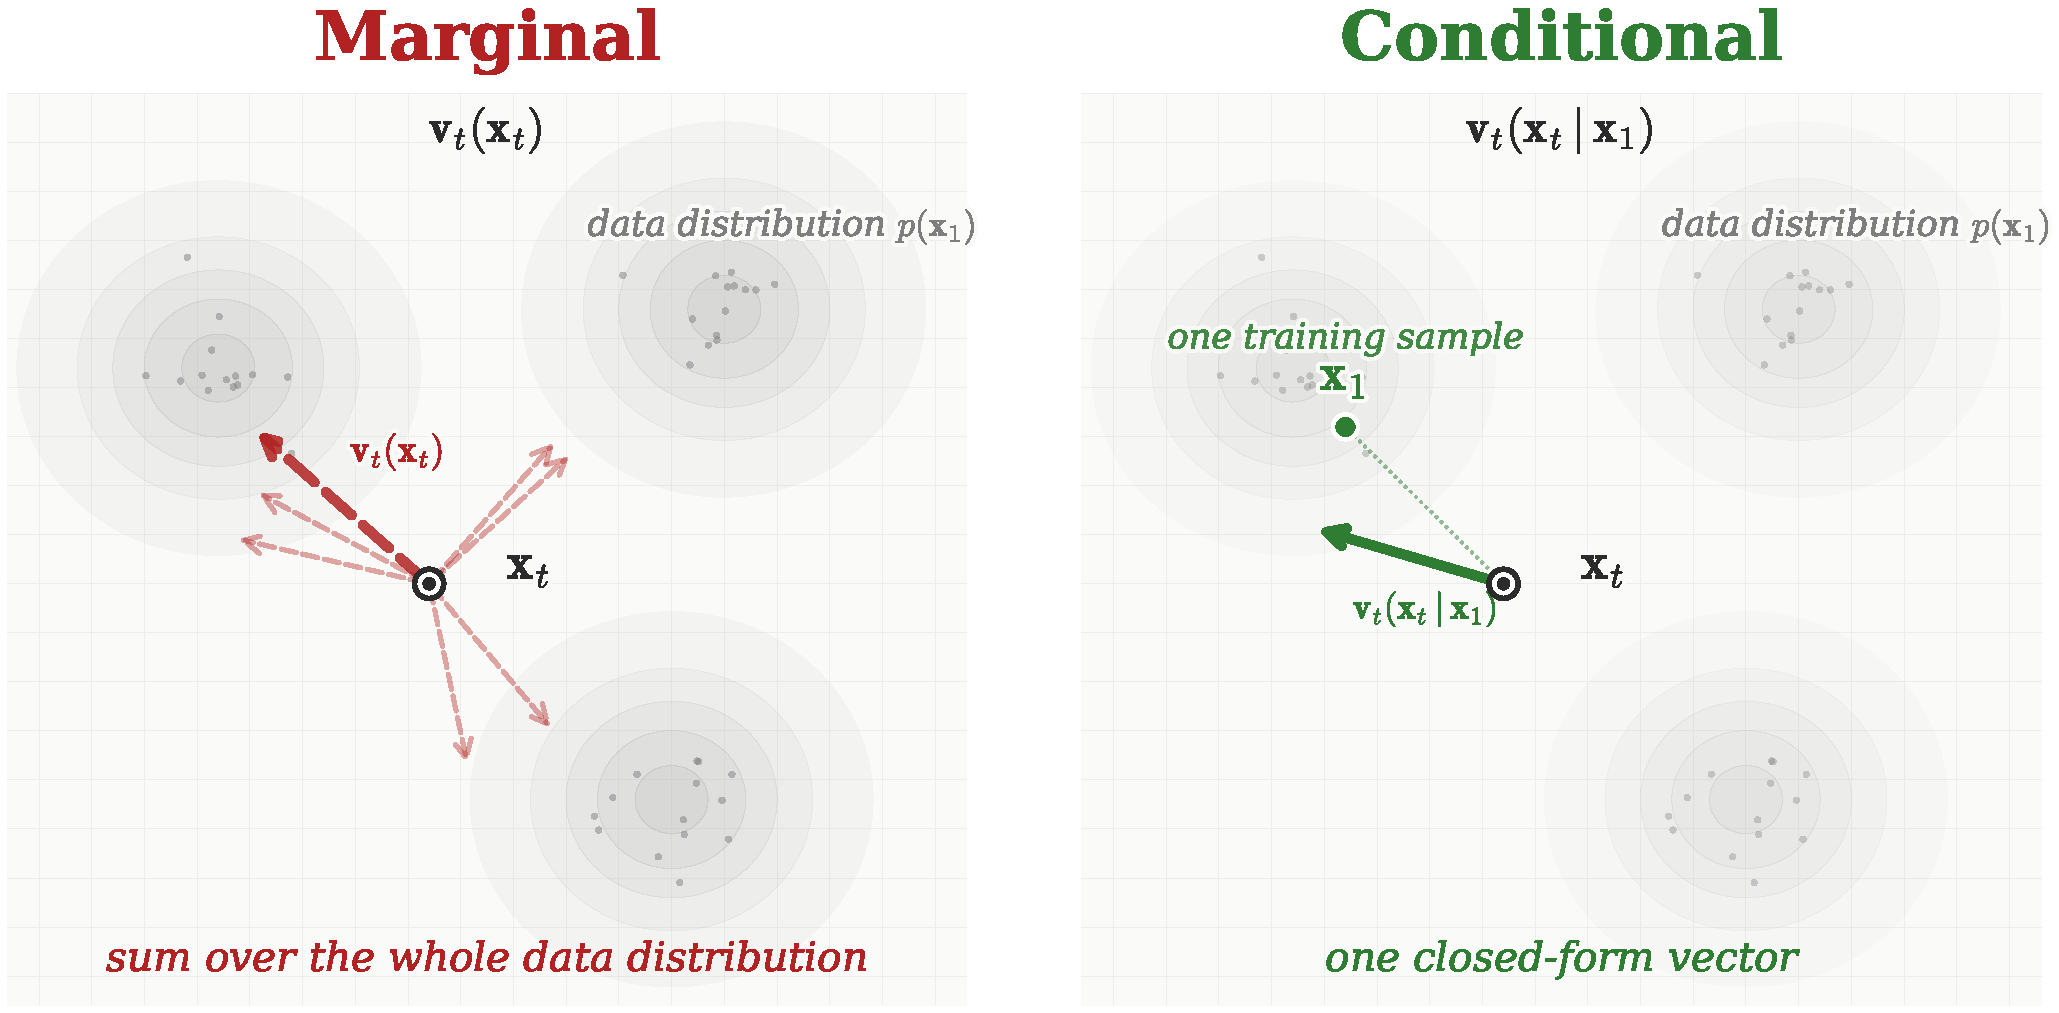
\includegraphics[width=\linewidth]{Images/PartB/flow_matching_conditional.pdf}
    \caption{\textbfs{流匹配中的条件技巧。}
    这里，$\rvx_1\sim p_{\mathrm{tgt}}$表示目标数据样本。
    \textbfs{(左)}
    对于固定中间样本 $\rvx_t$，边缘速度
    $\rvv_t(\rvx_t)$ 平均与相关的条件速度
    所有可能产生的目标样本 $\rvx_1$
    $\rvx_t$。每个 $\rvx_1$ 的贡献按以下方式加权
    它与观察到的 $\rvx_t$ 兼容。计算这个平均值
    直接需要对整个目标分布进行积分，并且
    一般是很难处理的。
    \textbfs{(右)}
    然而，在训练过程中，使用了特定的目标样本 $\rvx_1$
    构造$\rvx_t$是已知的。对该样本进行调节可以得出
    闭式速度 $\rvv_t(\rvx_t|\rvx_1)
        =
        b_t'\rvx_1
        +
        \frac{a_t'}{a_t}
        \bigl(\rvx_t-b_t\rvx_1\bigr)$，
    它提供一个简单的向量作为回归目标
    （提案~\ref{closed-form-vf}）。虽然每个训练示例
    仅针对一个目标样本的条件，对条件进行平均
    对数据的训练目标给出了相同的最佳边缘
    速度场；参见定理~\ref{thm:fm-cfm}。因此，条件流
    匹配学习 $\rvv_t(\rvx_t)$ 而无需直接回归
    通常难以处理的边缘速度。这是同样的条件
    变分透视中使用的原理
    (Theorem~\ref{thm:equiv-marginal-kl}) 和去噪分数匹配
    （定理~\ref{thm:sm-dsm}）。
    \figcredit{由作者使用AI辅助编码创建。}}
    \label{fig:cfm-illustration}
\end{figure}


我们将上述讨论总结如下：
\thmp{ $\mathcal{L}_{\mathrm{FM}}$ 和 $\mathcal{L}_{\mathrm{CFM}}$}{fm-cfm}{ 的等效项
以下内容成立：
\begin{align*}
    \mathcal{L}_{\mathrm{FM}}(\bm{\phi}) = \mathcal{L}_{\mathrm{CFM}}(\bm{\phi}) + C,
\end{align*}
其中 $C$ 是与参数 $\bm{\phi}$ 无关的常数。此外，两个损耗的最小者 $\rvv^*$ 满足
\[
    \rvv^*(\rvx_t, t) = \rvv_t(\rvx_t), \quad \text{for almost every } \rvx_t \sim p_t,
\]
其中 $\rvv_t(\rvx_t)$ 在 \Cref{eq:marginal-oracle-velocity} 中定义。
}{最小化器的论证和推导遵循与命题~\ref{dsm-minimizer}的分数匹配情况完全相同的推理。
}

这标志着调节技巧产生易于处理的训练目标的第三个实例，如 \Cref{fig:cfm-illustration} 中所示。值得注意的是，变分、基于分数和基于流程的方法都反映了相同的基本原理。\rmkb{
取$\pi = p_{\mathrm{data}}$，我们可以应用贝叶斯规则：
\[
p(\rvx_0|\rvx_t) = \frac{p_t(\rvx_t|\rvx_0) p_{\mathrm{data}}(\rvx_0)}{p_t(\rvx_t)},
\]
\Cref{eq:marginal-oracle-velocity} 的类似分解出现在基于分数的模型中：
\begin{align*}
    \nabla_{\rvx_t} \log p_t(\rvx_t) 
    &= \mathbb{E}_{\rvx_0 \sim p(\cdot|\rvx_t)} \left[ \nabla_{\rvx_t} \log p_t(\rvx_t|\rvx_0) \right] \\
    &= \mathbb{E}_{\rvx_0 \sim p_{\text{data}}} \left[ \nabla_{\rvx_t} \log p_t(\rvx_t|\rvx_0) \cdot \frac{p_t(\rvx_t|\rvx_0)}{p_t(\rvx_t)} \right],
\end{align*}
这反映了\Cref{eq:marginal-oracle-velocity}中的边缘化策略。
}

如在 \Cref{subsec:lesson-score} 中，必须明确指定条件密度 $p_t(\rvx_t|\rvz)$ 和条件速度场 $\rvv_t(\rvx_t|\rvz)$，对于 $p_t(\rvx_t|\rvx_0) = \mathcal{N}(\rvx_t; \alpha_t \rvx_0, \sigma_t^2 \rmI)$ 和 $\rvv_t(\rvx_t|\rvx_0) = f(t)\rvx_t - \frac{1}{2}g^2(t)\nabla_{\rvx_t} \log p_t(\rvx_t|\rvx_0)$，通用条件流匹配框架也需要这两个组件。然而，在这种一般情况下，我们还没有构造条件密度 $p_t(\rvx_t|\rvz)$ 或条件速度场 $\rvv_t(\rvx_t|\rvz)$。在\Cref{sec:instance-fm}中，我们介绍了这些组件的几个常见实例。


\subsection{扩散模型、一般流匹配与NODE的比较}\label{subsec:compare-dm-general-fm}


\paragraph{扩散模型与一般流动匹配的比较.}
\Cref{subsec:lesson-score} 的见解导致了一个扩展的 FM 框架，该框架保留了相同的基本原理。为了突出它们的相似之处，我们将它们总结在 \Cref{tab:framework_comparison} 中。


\begin{table}[th]
\caption{扩散模型（或高斯FM）与通用FM框架之间的比较。  
这里，一般的FM框架是指具有两侧调节的设置， 
其中 $\mathbf{x}_0 \sim p_{\text{src}}$ 和 $\mathbf{x}_1 \sim p_{\text{tgt}}$ 
独立采样。}
\label{tab:framework_comparison}
\centering
\resizebox{\textwidth}{!}{
\begin{tabular}{lcc}
\toprule
\textbfs{Aspect} & \textbfs{(基于分数)扩散模型} & \textbfs{通用 FM} \\
\midrule
源区$p_{\mathrm{src}}$ & 高斯先验 & 任何 \\
目标距离$p_{\mathrm{tgt}}$ & 数据分发 & 任意 \\
潜伏区$\pi(\rvz)$ & $p_{\text{data}}$ & 参见 \Cref{subsec:fm-instantiations} \\ 
条件。区。 $p_t(\rvx_t|\rvz)$ & $\mathcal{N}(\rvx_t;\alpha_t\rvx_0,\sigma_t^2\rmI)$ & 参见 \Cref{subsec:fm-instantiations} \\
边缘距离$p_t(\rvx_t)$ & $\int p_t(\rvx_t|\rvx_0) p_{\mathrm{data}}(\rvx_0) \diff\rvx_0$ & $ \int p_t(\rvx_t|\rvz) \pi(\rvz) \diff\rvz$ \\
条件。速度 $\rvv_t(\rvx|\rvz)$ & $f(t) \rvx - \frac{1}{2} g^2(t) \nabla \log p_t(\rvx|\rvx_0)$ & 参见 \Cref{subsec:fm-instantiations} \\
边缘速度 $\rvv_t(\rvx)$ & $f(t) \rvx - \frac{1}{2} g^2(t) \nabla \log p_t(\rvx)$ & 参见 \Cref{eq:marginal-oracle-velocity} \\
学习目标 & $\mathcal{L}_{\text{SM}}=\mathcal{L}_{\text{DSM}}+C$ & $\mathcal{L}_{\mathrm{FM}}=\mathcal{L}_{\mathrm{CFM}}+C$ \\
基本规则 & \multicolumn{2}{c}{Fokker-Planck / 连续性方程} \\
\bottomrule
\end{tabular}
}
\end{table}
我们注意到，假设高斯调度满足扩散-SDE
Lemma~\ref{forward-sde}中的兼容性条件，高斯FM本质上是
相当于相应的扩散公式（更多信息请参见
\Cref{ch:all-equivalent}）；因此我们不区分它们
除非明确说明。

\paragraph{与节点的连接。}
FM 可以被视为 NODE 的免仿真替代方案，在 \Cref{subsec:NODE}。虽然 CNF 需要在最大似然训练期间求解 ODE，这是计算密集型的，但 FM 通过简单的回归损失直接回归指定的速度场，从而绕过了这一点。关键的见解是，当连接源分布和目标分布的边缘密度路径固定时，训练期间的精确模拟就变得不必要了。


\subsection{（选读）基本结论}\label{subsec:fm-theory}

\paragraph{连续性方程：质量守恒定律。}  
类似于 PF-ODE 和 Fokker–Planck 分析 \Cref{subsec:lesson-score}，我们现在提出一个标准来验证 ODE 流引起的密度路径是否与规定路径对齐 $\{p_t\}_{t \in [0,1]}$。考虑描述随时间变化的速度场下粒子流动的常微分方程 $\rvv_t$:
\[
\frac{\diff \rvx(t)}{\diff t} = \rvv_t\left(\rvx(t)\right).
\]
如 \Cref{eq:pushforward-ode}，这个ODE定义了一个流映射 
$\bm{\Psi}_{s\to t}(\rvx_0)$ 对于任何 $s,t \in [0,1]$，特别是传输初始点 $\rvx_0 \sim p_{\mathrm{src}}$ 当时 $0$ 当时的状态 $t$。时间上的诱导分布 $t$ 由前推给出
\begin{align}\label{eq:ode-pushforward}
    p_t^{\mathrm{fwd}}(\rvx) 
    = \int \delta \left(\rvx - \bm{\Psi}_{0\to t}(\rvx_0)\right) 
      p_{\mathrm{src}}(\rvx_0) \mathrm{d}\rvx_0=: \bm{\Psi}_{0\to t}\# p_{\mathrm{src}},
\end{align}
这样 $\bm{\Psi}_{0\to t}(\rvx_0) \sim p_t^{\mathrm{fwd}}$ 每当 
$\rvx_0 \sim p_{\mathrm{src}}$。类似地，我们可以从 $\rvx_1 \sim p_{\mathrm{tgt}}$ 
至 $p_{\mathrm{src}}$ 通过 $\bm{\Psi}_{1\to 0}(\rvx_1)$。假设我们有一条规定的密度路径 $\{p_t\}_{t \in [0,1]}$，我们构造一个速度场 $\{\rvv_t\}_{t \in [0,1]}$ 定义粒子流。这自然会提出一个问题：

\begin{question}
    什么条件下流致密度 $p_t^{\mathrm{fwd}}$  与目标密度完全匹配 $p_t$ 对于所有 $t \in [0,1]$?
\end{question}
一旦两种密度演化一致，我们就可以利用 ODE 流程在两者之间灵活传输样本 $p_{\mathrm{src}}$ 和 $p_{\mathrm{tgt}}$ 通过求解 ODE。如在 \Cref{eq:p_t-fwd-rev}，验证这种对齐的原则方法是通过 \emph{连续性方程}，它捕获了随时间演化的密度中的质量守恒：

\thmp{质量守恒准则}{continuity-mass}{
流致密度 $p_t^{\mathrm{fwd}}$ 等于规定路径 $p_t$ 对于所有 $t \in [0,1]$; i.e., 
\[
p_t^{\mathrm{fwd}} = p_t, \quad \text{for all } t \in [0,1],
\]
当且仅当该对 $(p_t, \rvv_t)$  满足连续性方程：
\[
\partial_t p_t(\rvx) + \nabla_\rvx \cdot (p_t(\rvx) \rvv_t(\rvx)) = 0,
\]
对于所有 $t\in[0,1]$ 和 $\rvx$.
}{概念推导提供于 \Cref{app-sec:mass-conservation}，而更严格的处理可以在 \citep{villani2008optimal} （参见“质量守恒公式”）。}

\paragraph{从条件路径到边缘路径。} 如所示 \Cref{subsec:fm-framework}，我们首先定义条件概率路径 $p_t(\cdot| \rvz)$ 以及相应的条件速度场 $\rvv_t(\cdot| \rvz)$。然后我们通过以下方式构建边缘速度场：
\[
    \rvv_t(\rvx) 
    = \int \rvv_t(\rvx| \rvz) \frac{p_t(\rvx| \rvz) \pi(\rvz)}{p_t(\rvx)}   \diff \rvz,
\]
如 \Cref{eq:marginal-oracle-velocity}。然而，我们仍然需要确保最终的边缘速度 $\rvv_t$ 引发密度路径与规定一致的 ODE 流 $p_t$。幸运的是，这种验证可以完全在条件级别完成：如果每个条件速度场 $\rvv_t(\cdot| \rvz)$ 诱导条件密度路径 $p_t(\cdot| \rvz)$，则得到的边缘速度 $\rvv_t$ 也导出正确的边缘路径。形式上，我们给出下面的结果，并在一个地方提供完整的推导，以明确地显示边缘速度场如何采用这种形式：

\proppp{边缘 VF 生成给定的边缘密度}{marginal-vf}{
如果条件速度场 $\rvv_t(\cdot|\rvz)$ 诱导匹配的条件密度路径 $p_t(\cdot|\rvz)$ （从 $p_0(\cdot|\rvz)$)，则边缘速度场 $\rvv_t(\cdot)$ 定义于 \Cref{eq:marginal-oracle-velocity} 产生与 $p_t(\cdot)$，从 $p_0(\cdot)$.
}{
通过验证该对得出此结果 $(p_t, \rvv_t)$ 满足连续性方程。我们以相反的方式提出论证，以直观地解释为什么边缘化速度场采用以下形式： \Cref{eq:marginal-oracle-velocity}。由于条件速度场 $\rvv_t(\cdot|\rvz)$ 诱导与条件密度匹配的密度路径 $p_t(\cdot|\rvz)$ 用于 $\rvz \sim \pi$，连续性方程对于每个条件对都成立：
\begin{align}\label{eq:continuity_conditional_pt}
    \frac{\diff}{\diff t} p_t(\rvx|\rvz) =- \nabla_\rvx \cdot \big(\rvv_t(\rvx|\rvz) p_t(\rvx|\rvz)\big).
\end{align}
我们的目标是找到速度场 ${\color{orange}\rvv_t(\cdot)}$ 其诱导密度与边缘密度一致 $p_t$，即满足
\begin{align}\label{eq:p_t_continuity}
    \frac{\diff}{\diff t} p_t(\rvx) =- \nabla_\rvx \cdot \big({\color{orange}\rvv_t(\rvx)} p_t(\rvx)\big).
\end{align}
从定义开始 $p_t$ 在 \Cref{eq:p_t}, 
\begin{align*}
  \frac{\diff}{\diff t} p_t(\rvx) &=\int \frac{\diff}{\diff t} p_t(\rvx_t|\rvz)\pi(\rvz)\diff \rvz \nonumber\\
  &=  - \int \nabla_\rvx \cdot\Big(  \rvv_t(\rvx|\rvz) p_t(\rvx | \rvz)  \Big)\pi(\rvz) \diff \rvz \quad \nonumber \\
  &=  -\nabla_\rvx \cdot \Big( \int  \rvv_t(\rvx|\rvz) p_t(\rvx | \rvz) 
 \pi(\rvz) \diff \rvz\Big), \nonumber  
\end{align*}
第二个等式遵循应用 \Cref{eq:continuity_conditional_pt}。将此与右侧进行比较 \Cref{eq:p_t_continuity} 表明，直到无散项，
\[
    {\color{orange}\rvv_t(\rvx)} p_t(\rvx) = \int \rvv_t(\rvx|\rvz) p_t(\rvx|\rvz) \pi(\rvz) \diff \rvz.
\]
因此，我们可以定义
\[
    {\color{orange}\rvv_t(\rvx)} := \int \rvv_t(\rvx|\rvz) \frac{p_t(\rvx|\rvz)}{p_t(\rvx)} \pi(\rvz) \diff \rvz,
\]
这正是以下形式 \Cref{eq:marginal-oracle-velocity}。该定理的证明本质上遵循该论证的相反过程。
}

这种连接使我们能够减少潜在棘手的边缘速度场的构造，以定义更简单的条件场 $\rvv_t(\cdot| \rvz)$，通过构造更容易使用。




\newpage

\section{构建分布之间的概率路径和速度}\label{sec:instance-fm}流匹配的本质在于源分布逐渐转变为目标分布。为了指导这种转换，需要两个关键元素：\emph{概率路径} $p_{t}$，它提供了每个时间$t$演化分布的快照，以及\emph{速度场} $\rvv_{t}$，它描述了单个粒子如何沿着路径移动。这两个对象不是独立的；它们通过连续性方程联系起来，这确保了粒子动力学与分布的演化一致。因此，学习任务简化为寻找忠实驱动该过程的速度场 $\rvv_t$。然而，困难在于，对于一般和复杂的分布，真正的边缘速度 $\rvv_t$ 是未知的，这给我们留下了一个无法直接访问的棘手目标。 

条件流匹配的核心思想是通过构建人工但易于处理的过程来解决真实边缘速度的棘手问题。为此，我们引入条件变量 $\rvz$ 并设计条件速度 $\rvv_t(\rvx_t|\rvz)$ 和/或条件路径 $p_t(\rvx_t|\rvz)$，故意选择简单。

 由于这些条件对象以封闭形式已知，因此它们充当模型可以回归的代理目标。如果满足两个实际要求，这会导致有效的训练损失 $\mathcal{L}_{\mathrm{CFM}}$：（i）我们可以从 $p_t(\cdot|\rvz)$ 中有效采样，以及（ii）相应的速度 $\rvv_t(\cdot|\rvz)$ 允许封闭式表达式。 


我们应该如何设计一个行为良好的条件过程？为了获得灵感，我们转向一个完全理解的案例：高斯到高斯桥 (\Cref{subsec:special-fm-instantiations})。这个例子强调了两种自然的设计策略：每次采用高斯概率路径 $t$，或者规定仿射速度场，这两种策略在分析上都是易于处理的。 







在这种见解的指导下，我们使用以下方法扩展到通用端点分布
两个互补的构造视图（另见
\Cref{subsec:cov-continuity-eq}）。这些对应经典
运输的欧拉和拉格朗日描述：

\begin{itemize}
    \item \textbfs{条件概率-路径优先（欧拉视图）.}
    我们从条件密度路径开始
    $p_t(\cdot|\rvz)$ 并求条件速度场
    $\rvv_t(\cdot|\rvz)$ 满足连续性方程。自从一个
    单独的密度路径通常不能确定唯一的速度，
    这种结构还需要选择一个特定的兼容
    速度场。

    \item \textbfs{条件流优先（拉格朗日视图）.}
    相反，我们指定单个粒子如何通过条件移动
    流映射$\bPsi_{0\to t}(\cdot|\rvz)$。获得诱导密度
    通过前推，并且当流映射可逆时，相应的
    欧拉速度场为
    \[
    \rvv_t
    =
    \partial_t\bPsi_{0\to t}
    \circ
    \bPsi_{0\to t}^{-1}.
    \]
\end{itemize}

在 \Cref{subsec:fm-instantiations}，我们详细介绍了第一种方法，该方法显示了其与中讨论的扩散模型构造的密切相似性 \Cref{subsec:lesson-score}，在 \Cref{subsec:prob-path-flow} 我们介绍第二个。这些观点共同提供了一个实用的框架来定义 $p_t(\rvx_t| \rvz)$ 和 $\rvv_t(\rvx_t| \rvz)$，实现无模拟训练以及任意源分布和目标分布之间的流构建。





\subsection{一个关键的特殊情况：边缘 $p_t(\rvx_t)$ 和速度 $\rvv_t(\rvx_t)$ 在高斯到高斯桥中}\label{subsec:special-fm-instantiations}

我们从高斯端点情况开始，我们可以计算边缘密度 $p_t(\rvx_t)$ 和速度场 $\rvv_t(\rvx_t)$ 分析性的。这作为条件密度的一般构造的模板 $p_t(\rvx_t |\rvz_t)$ 和速度场 $\rvv_t(\rvx_t |\rvz_t)$。当源和目标分布时， $p_{\text{src}}$ 和 $p_{\text{tgt}}$，均为高斯分布，速度场 $\rvv_t(\cdot)$ 允许封闭式表达式。我们考虑插值边缘密度路径：
\begin{align}\label{eq:gaussian-density-path}
    p_t(\rvx_t) = \mathcal{N}\left(\rvx_t; \bm{\mu}(t), \sigma^2(t) \rmI\right),
\end{align}
随时间变化的均值 $\bm{\mu}(t)$ 和方差 $\sigma^2(t)>0$。两个端点由下式给出
\[
p_{\text{src}} = p_0 =  \mathcal{N}\left(\rvx; \bm{\mu}(0), \sigma^2(0) \rmI\right), \quad
p_{\text{tgt}} = p_1 =  \mathcal{N}\left(\rvx; \bm{\mu}(1), \sigma^2(1) \rmI\right),
\]
这样路径 $\{p_t\}_{t \in [0,1]}$ 连接这些发行版。使用给定的路径 $\{p_t\}_{t \in [0,1]}$，确实有很多速度场会引发 ODE 流 $\bm{\Psi}_{0\to t}(\rvx)$ 这样 $\rvx \sim p_0$ 暗示 $\bm{\Psi}_{0\to t}(\rvx) \sim p_t$。对于这个高斯路径，一个特别简单的实现由下式给出\footnote{在 \citep{lipman2022flow}，作者认为 $\bm{\Psi}_{0\to t}(\rvx) = \bm{\mu}(t) + \sigma(t)\rvx$，这需要约束 $\bm{\mu}(t)$ 和 $\sigma(t)$ 保证边界条件。我们采用等效的标准化公式来避免此类限制。}:
\begin{align}\label{eq:gaussian-sol-map}
    \bm{\Psi}_{0\to t}(\rvx) := \bm{\mu}(t) + \sigma(t) \left( \frac{\rvx - \bm{\mu}(0)}{\sigma(0)} \right).
\end{align}

对于定义的高斯路径 $p_t$ （所有的高斯 $t$)，速度场 $\rvv_t(\cdot)$ 引入 ODE 流 \Cref{eq:gaussian-sol-map} 具有独特的分析特征如下~\citep{lipman2022flow}:

\proppp{高斯密度路径的封闭式速度场}{closed-form-vf}{
让 $p_t$ 是高斯路径 \Cref{eq:gaussian-density-path}。那么速度场 $\rvv_t(\cdot)$ 生成 ODE 流 \Cref{eq:gaussian-sol-map} 对于定义的来说是唯一的 $\bPsi_{0\to t}$ 并且具有闭合形式表达式：
\begin{equation*}
    \rvv_t(\rvx) = \frac{\sigma'(t)}{\sigma(t)} \left( \rvx - \bm{\mu}(t) \right) + \bm{\mu}'(t).
\end{equation*}
}{考虑具有初始条件的 ODE $\rvy$:
\[
    \frac{\diff}{\diff t} \bm{\Psi}_{0\to t}(\rvy) = \rvv_t(\bm{\Psi}_{0\to t}(\rvy)).
\]
自 $\bm{\Psi}_{0\to t}$ 是可逆的（如 $\sigma(t)>0$)，我们可以设置 $\rvx = \bm{\Psi}_{0\to t}(\rvy)$ 和 $\rvy = \bm{\Psi}_{0\to t}^{-1}(\rvx) = \bm{\Psi}_{t\to 0}(\rvx)$ 获取
\[
    \bm{\Psi}_{0\to t}'\big(\bm{\Psi}_{0\to t}^{-1}(\rvx)\big) = \rvv_t(\rvx).
\]
区分 \Cref{eq:gaussian-sol-map} 相对于 $t$ 给出
\begin{equation*}
    \bm{\Psi}_{0\to t}'(\rvx) = \bm{\mu}'(t) + \sigma'(t) \left( \frac{\rvx - \bm{\mu}(0)}{\sigma(0)} \right).
\end{equation*}
解决 $\rvy = \bm{\Psi}_{0\to t}^{-1}(\rvx)$ 产量
\[
    \rvy = \bm{\mu}(0) + \sigma(0) \left( \frac{\rvx - \bm{\mu}(t)}{\sigma(t)} \right).
\]
将其代入 $\bm{\Psi}_{0\to t}'(\rvx)$ 给出
\[
    \rvv_t(\rvx) = \frac{\sigma'(t)}{\sigma(t)} \left( \rvx - \bm{\mu}(t) \right) + \bm{\mu}'(t),
\]
如所声称的那样。
}
我们注意到对于固定流图 $\bPsi_{0\to t}$ （流优先视图），速度由下式唯一确定
\[
\rvv_t  =  \partial_t \bPsi_{0\to t} \circ \bPsi_{0\to t}^{-1}.
\]
在这种结构下，这对 $(p_t,\rvv_t)$ 自动满足连续性方程。相比之下，对于给定的密度路径 $t\mapsto p_t$ 无固定 $\bPsi_{0\to t}$ （概率路径优先视图），速度场不是唯一的。

这种区别准确地表征了流优先和概率路径优先观点之间的差异。当对潜变量进行调节时，这种封闭形式的表征仍然有效 $\rvz$。接下来，我们扩展这一见解来构建条件高斯路径 $p_t(\cdot|\rvz)$
并推导相应的条件速度场 $\rvv_t(\cdot|\rvz)$ 用于一般边缘设置。




\subsection{先构造条件概率路径 $\rvv_t(\cdot|\rvz)$ 和 $p_t(\cdot|\rvz)$}\label{subsec:fm-instantiations}


\begin{figure}[th!]
    \centering
    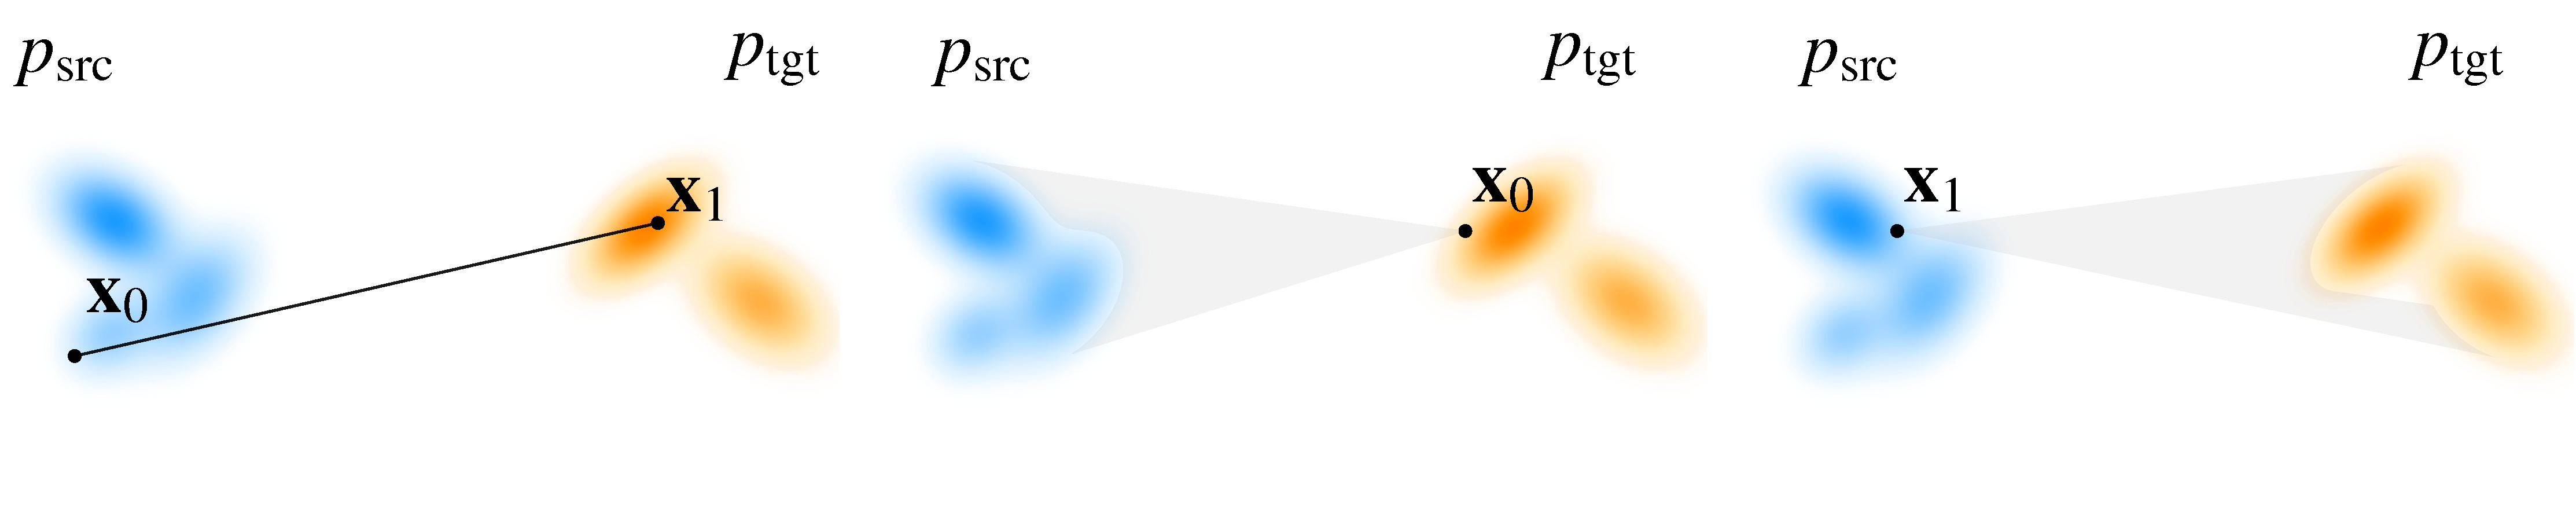
\includegraphics[width=\linewidth]{Images/PartB/triptych_gray_cones_final.pdf}
    \caption{\textbfs{两种常见类型的条件概率路径的图示}。它包括：（一） \emph{双面}，条件为 $\rvx_0 \sim p_{\text{tgt}}$ 和 $\rvx_1 \sim p_{\text{src}}$ 具有一般端点分布； (二) \emph{单面}，条件为 $\rvx_0 \sim p_{\text{tgt}}$ 或 $\rvx_1 \sim p_{\text{src}}$.
\figcredit{由作者创建。}}
    \label{fig:conditional-path}
\end{figure}

我们的目标是构建一条条件密度路径 $p_t(\cdot|\rvz)$ 先求出其对应的条件速度场 $\rvv_t(\cdot|\rvz)$ （通过提案~\ref{closed-form-vf}），在条件下 $\pi(\rvz)$。取决于如何 $\rvz$ 选择后，有两种自然情况：(i) 两侧调节 $\rvz=(\rvx_0,\rvx_1)$，或 (ii) 单侧调节 $\rvz=\rvx_0$ 或 $\rvx_1$。无论哪种情况，构造都必须匹配边界分布：
\begin{align*}
   p_{\mathrm{src}}(\rvx_0) = \int p_0(\rvx_0|\rvz) \pi(\rvz)\diff\rvz, \quad
   p_{\mathrm{tgt}}(\rvx_1) = \int p_1(\rvx_1|\rvz) \pi(\rvz) \diff\rvz.
\end{align*}
由于一旦指定了具体结构，验证这些约束就很简单，因此我们在这里不强调验证步骤。


 
\paragraph{一、双面 $\rvz = (\rvx_0, \rvx_1)$ —“光束状”路径。}
    \subparagraph{选择 $\pi(\rvz)$.} 考虑一般分布 $p_{\mathrm{src}}$ 和 $p_{\mathrm{tgt}}$ 结束 $\mathbb{R}^D$。让 $\rvz = (\rvx_0, \rvx_1)$ 与 $\rvx_0 \sim p_{\mathrm{src}}$ 和 $\rvx_1 \sim p_{\mathrm{tgt}}$ 独立，即
    \[
    \pi(\rvz) = p_{\mathrm{src}}(\rvx_0)  p_{\mathrm{tgt}}(\rvx_1).
    \]
    \subparagraph{条件路径的选择 $p_t(\cdot|\rvz)$.} 通过固定且小方差的线性插值定义条件路径 $\sigma > 0$\footnote{
可以添加固定条件方差 $\sigma^2\rmI$。条件速度保持不变 $a_t'\rvx_0+b_t'\rvx_1$ 因为方差在时间上是恒定的，但是端点边缘变成了高斯平滑 $p_{\mathrm{src}}$ 和 $p_{\mathrm{tgt}}$，接近所需的端点 $\sigma\to0$.
}:
    \[
    p_t(\rvx_t | \rvz = (\rvx_0, \rvx_1)) = \mathcal{N}(\rvx_t; a_t\rvx_0 + b_t\rvx_1,  \sigma^2 \rmI),
    \]
    其中 $a_t$ 和 $b_t$ 是满足时间相关的函数  $a_0 = 1,  b_0 = 0$ 和 $a_1 = 0,  b_1 = 1$。建议的选择 \citep{lipman2022flow,liu2022rectified} 是 $a_t = 1-t$, $b_t = t$。在确定性情况下 $\sigma = 0$，我们得到  
\[
p_t(\rvx_t |\rvz) = \delta \big(\rvx_t - [a_t\rvx_0 + b_t\rvx_1]\big),
\]
描述了从 $\rvx_0$ 至 $\rvx_1$.
    \subparagraph{导出条件速度  $\rvv_t(\cdot|\rvz)$.} 按提议~\ref{closed-form-vf}，条件速度为
    \[
    \rvv_t(\rvx | \rvz) = a'_t\rvx_0 + b'_t\rvx_1.
    \]
    \subparagraph{CFM 损失。} 当 $\sigma=0$ 这样 $\rvx_t = a_t\rvx_0 + b_t\rvx_1$，CFM 损失减少为
    \[
    \mathcal{L}_{\mathrm{CFM}} = \mathbb{E}_{t, \rvx_0\sim p_{\text{src}}, \rvx_1\sim p_{\text{tgt}}} \left\| \rvv_{\bm{\phi}}(\rvx_t, t) - \left(a'_t\rvx_0 + b'_t\rvx_1\right) \right\|^2.
    \]
来自 \Cref{eq:marginal-oracle-velocity,eq:minimum_velocity}，最优速度场为
\[
\rvv^*(\rvx_t, t) = \mathbb{E} \left[ \rvx_t'|\rvx_t \right] = \mathbb{E} \left[ a'_t\rvx_0 + b'_t\rvx_1|\rvx_t \right].
\]
在这里，期望被接管 $p(\mathbf{x}_0, \mathbf{x}_1|\mathbf{x}_t)$，源-目标对上的条件分布 $(\mathbf{x}_0, \mathbf{x}_1)$ 这可能会产生观察到的插值 $\mathbf{x}_t = a_t\mathbf{x}_0 + b_t\mathbf{x}_1$ 当时 $t$.



\paragraph{二。一面 $\rvz = \rvx_0$ 或 $\rvx_1$ —“聚光灯式”路径。}
我们说明了单边设置中的先构造条件概率路径，考虑到标准生成设置 $p_{\mathrm{src}}=\mathcal N(\bm 0,\rmI)$ 和 $p_{\mathrm{tgt}}=p_{\mathrm{data}}$。至关重要的是，这个高斯源不是一个额外的假设，而是下面定义的条件路径的直接结果。任意端点的更一般处理将在 \Cref{subsec:prob-path-flow}.

\subparagraph{选择 $\pi(\rvz)$.}
我们采取 $\rvz=\rvx_1$ 与 $\pi(\rvz)=p_{\mathrm{data}}(\rvx_1)$ （案例 $\rvz=\rvx_0\sim p_{\mathrm{prior}}$ 类似）。

\subparagraph{条件路径的选择 $p_t(\cdot|\rvz)$.}
用于固定 $\rvx_1\sim p_{\mathrm{data}}$, 定义
\[
p_t(\rvx_t|\rvz=\rvx_1)=\mathcal N \big(\rvx_t; b_t \rvx_1, a_t^2 \rmI\big),
\]
与 $ a_0=1, b_0=0, a_1=0, b_1=1$ （通常解释为限制）。在边界处，
\[
p_0(\cdot|\rvz=\rvx_1)=\mathcal N(\cdot; \bm 0,\rmI),\qquad
p_1(\cdot|\rvz=\rvx_1)=\delta(\cdot - \rvx_1).
\]
边缘化 $\rvx_1$ 产量 $\{p_t\}_{t\in[0,1]}$ 与
$p_0=\mathcal N(\bm 0,\rmI)$ （独立于 $p_{\mathrm{data}}$) 和 $p_1=p_{\mathrm{data}}$.

\subparagraph{导出条件速度  $\rvv_t(\cdot|\rvz)$.}
对于 $t\in(0,1)$ 与 $a_t>0$，应用命题~\ref{closed-form-vf} 条件高斯路径给出
\[
\mathbf v_t(\rvx|\rvx_1)
= b_t' \rvx_1 + \frac{a_t'}{a_t} \big(\rvx - b_t \rvx_1\big).
\]

\subparagraph{单侧 CFM 物镜。}
有 $t\sim\mathcal U(0,1)$ （或任何固定抽样分布）和 $\rvx_1\sim p_{\mathrm{data}}$，CFM 损失变为
\begin{align}\label{eq:one-sided-cfm}
    \mathcal L_{\mathrm{CFM}}
=\E_{t,\rvx_1} \E_{\rvx_t\sim p_t(\cdot|\rvx_1)}
\Big\|\mathbf v_\phi(\rvx_t,t)-
\Big[b_t'\rvx_1+\tfrac{a_t'}{a_t}\big(\rvx_t-b_t\rvx_1\big)\Big]\Big\|_2^2.
\end{align}
通过MSE最优性，唯一的极小值是边缘速度场
\[
\mathbf v^*(\rvx,t)
= \E \left[\mathbf v_t(\rvx|\rvx_1) |dle|  \rvx_t=\rvx\right]
= \E \left[a_t'\rvx_0+b_t'\rvx_1 |dle|  \rvx_t=\rvx\right].
\]

\subparagraph{相当于两侧目标。}
用于配对样品 $(\rvx_0,\rvx_1)$ 与 $\rvx_t=a_t\rvx_0+b_t\rvx_1$,
\[
\mathbf v_t(\rvx_t|\rvx_1)
= b_t'\rvx_1 + \tfrac{a_t'}{a_t}\big(\rvx_t-b_t\rvx_1\big)
= a_t'\rvx_0 + b_t'\rvx_1.
\]
因此单边损失回归到 \emph{条件期望} 给定的两侧目标 $\rvx_t$:
\[
\mathbf v^*(\rvx,t)=\E \big[a_t'\rvx_0 + b_t'\rvx_1 | \rvx_t=\rvx\big],
\]
因此单面和双面 CFM 物镜共享相同的最小化器。


\paragraph{高斯 FM = 扩散模型。}
我们使用 FM 约定，其中 $t=0$ 表示源/先验和 $t=1$ 表示目标/数据：
\[
p_{\mathrm{src}}=p_{\mathrm{prior}},\qquad p_{\mathrm{tgt}}=p_{\mathrm{data}}.
\]
相比之下，扩散模型通常索引从数据到噪声的时间（即， $t=0$ 是数据并且 $t=1$ 优先）。这里，我们主要讨论采用FM约定索引。然而，为了比较，VE 和 VP 条目 \Cref{tb:interpolant_instances} 在通常的扩散时间索引中进行了总结，其中 $t=0$ 对应数据和 $t=1$ 先验/噪声。如果进一步 $p_{\mathrm{src}}=\mathcal N(\bm 0,\rmI)$，则对于固定条件 $\rvx_1\sim p_{\mathrm{data}}$，条件路径 $p_t(\cdot |\rvx_1)$ 自然选择高斯分布，而目标分布 $p_{\mathrm{tgt}}$ 本身不需要是高斯的。我们将此高斯条件路径设置称为 \emph{高斯调频}。扩散概率路径形成了此类高斯路径的重要子类。然而，通用高斯调度不需要对应于有效的前向扩散 SDE；该时间表还必须满足引理中的 SDE 兼容性条件~\ref{forward-sde}。选择 $a_t = 1-t$ 和 $b_t = t$ （相当于， $\alpha_t = t$ 和 $\sigma_t = 1-t$ 正在重新贴标 $a_t:=\sigma_t$, $b_t:=\alpha_t$ 在扩散模型中）恢复熟悉的 FM/RF 时间表~\citep{lipman2022flow,liu2022rectified}.


\begin{table}[th]
\caption{不同插值的总结写为
$\rvx_t=a_t\rvx_0+b_t\rvx_1$，其中
$\rvx_0\sim p_{\mathrm{src}}=p_{\mathrm{prior}}$ 和
$\rvx_1\sim p_{\mathrm{tgt}}=p_{\mathrm{data}}$。 FM/RF 和三角列使用 FM 约定（$t=0$ 来源， $t=1$ 目标），而 VE/VP 色谱柱保留了通常的扩散时间约定（$t=0$ 数据， $t=1$ 先验/噪声），其中
$a_t:=\sigma_t$ 和 $b_t:=\alpha_t$。对于有限终端噪声水平下的 VE，精确的终端边缘为
$p_{\mathrm{data}}*\mathcal{N}(\bm{0},a_1^2\rmI)$;表中所示的高斯先验是当终端噪声主导数据规模时的通常近似值。}
  \small
  \centering
  \resizebox{\textwidth}{!}{
  \begin{tabular}{lcccc}
     \toprule
         & \textbfs{VE} & \textbfs{副总裁} & \textbfs{调频/射频} & \textbfs{触发。}~\citep{albergo2023stochastic} \\
    \midrule
     $a_t$ （先验系数） 
       & $a_t$ 
       & $\sqrt{1-b_t^2}$ 
       & $1-t$ 
       & $\cos \bigl(\tfrac{\pi}{2}t\bigr)$ \\
     $b_t$ （数据系数） 
       & $1$ 
       & $b_t$ 
       & $t$ 
       & $\sin \bigl(\tfrac{\pi}{2}t\bigr)$ \\
    \midrule
     $a_0$ & $0$ & $0$ & $1$ & $1$ \\
     $b_0$ & $1$ & $1$ & $0$ & $0$ \\
     $a_1$ & $a_1$ & $1$ & $0$ & $0$ \\
     $b_1$ & $1$ & $0$ & $1$ & $1$ \\
    \midrule
     $p_{\text{prior}}$ 
       & $p_{\mathrm{data}} * \mathcal{N}(\bm{0},a_1^2\rmI)
   \approx \mathcal{N}(\bm{0},a_1^2\rmI)$ 
       & $\mathcal{N}(\bm{0},\rmI)$ 
       & $\mathcal{N}(\bm{0},\rmI)$ 
       & $\mathcal{N}(\bm{0},\rmI)$ \\
     \bottomrule
  \end{tabular}}
  \label{tb:interpolant_instances}
\end{table}



在高斯 FM 设置中，光束状和聚光灯状条件路径都会导致与标准扩散损失类似的训练目标。正如我们将在 \Cref{ch:all-equivalent}，高斯FM实际上可以等价地解释为一个训练来预测的扩散模型 \emph{速度}，在线性计划下 $a_t = 1-t$ 和 $b_t = t$。这一观点强调，流动匹配和扩散并没有本质上的不同，而是两种可以相互转化的等效公式。高斯 FM 目标在实践中特别有吸引力：它的损失函数 ($\E_{t,\rvx_t} \left[\norm{\rvv_\bphi(\rvx_t, t) - (\rvx_1 - \rvx_0)}_2^2\right]$) 很简单，并且已被证明可以在规模上实现有竞争力的性能~\citep{esser2024scaling}. 




\subsection{先构造条件流 $\rvv_t(\cdot|\rvz)$ 和 $p_t(\cdot|\rvz)$}\label{subsec:prob-path-flow}

我们处理端点的一般情况 $p_{\mathrm{src}}$ （在 $t=0$) 和 $p_{\mathrm{tgt}}$ （在 $t=1$) 是任意的。我们的目标是直接在轨迹空间中设计一个条件流，将样本从 $p_{\mathrm{src}}$ 至 $p_{\mathrm{tgt}}$ 并产生封闭形式 $\rvv_t(\rvx_t|\rvz)$ 可用作回归目标。

\paragraph{动机。}
我们可以直接指定条件流映射，而不是首先设计条件密度路径 $\bPsi_{0\to t}(\cdot;\rvz)$ 沿着轨迹移动样本。这有两个实际优点：（i）它通过沿轨迹的时间导数立即产生用于训练的回归目标； (ii) 在几何结构空间（黎曼流形、李群或约束子流形）上，构造条件流映射通常是很自然的 
$\bPsi_{0\to t}$ 直接来自几何（例如，测地线、指数图或预测几何）~\citep{lipman2024flow} 生成用于训练的分析、免模拟目标速度。


\paragraph{条件仿射流（命题链接~\ref{closed-form-vf}).}
我们修复条件变量 $\rvz\sim\pi$ (e.g., $\rvz=\rvx_1\sim p_{\mathrm{tgt}}$ 在片面的“聚光灯”训练中）并向前推进 $\rvx_0\sim p_{\mathrm{src}}$ 通过时变 \emph{条件仿射流} 
\[
\bPsi_{0\to t}(\rvx_0;\rvz) := \bm\mu_t(\rvz) + \rmA_t(\rvz) \rvx_0,\qquad t\in[0,1],
\]
其中 $\bm\mu_t(\rvz)\in\R^D$ 和 $\rmA_t(\rvz)\in\R^{D\times D}$ 可逆 $t\in(0,1)$。边界 
$\rmA_0(\rvz)=\rmI,\ \bm\mu_0(\rvz)=\mathbf 0$ 恢复 $p_{\mathrm{src}}$ 在 $t=0$。解释边界的标准是 $t\to1$ 作为限制（终端映射可能将质量集中在较低维的集合或点上）\footnote{允许 $\rmA_1(\rvz)$ 为单数（例如， $\mathbf 0$) 与可逆性兼容 $(0,1)$ 并导致路径收缩到指定端点 $t=1$.}. 


\subparagraph{诱导条件路径 $p_t(\cdot|\rvz)$.}
结构定义
\[
p_t(\cdot|\rvz) = \bigl(\bPsi_{0\to t}( \cdot ;\rvz)\bigr)_{\#} p_{\mathrm{src}},
\qquad
p_t(\cdot)  =  \int p_t(\cdot|\rvz)\pi(\rvz)\diff\rvz.
\]
最终重要的是 $\mathcal{L}_{\mathrm{CFM}}$ 如何从中采样：第一次绘制 $\rvz \sim \pi$，然后画 $\rvx_0 \sim p_{\mathrm{src}}$，最后设置
\[
\rvx_t = \bm\mu_t(\rvz) + \rmA_t(\rvz)\rvx_0.
\]


我们注意到，当 $\bPsi_{0\to t}$ 仿射于 $\rvx_0$，那么 $p_t( \cdot | \rvz)$ 是高斯分布当且仅当 $p_{\mathrm{src}}$ 是高斯分布。特别是对于任意（非高斯） $p_{\mathrm{src}}$，仿射流产生一般非高斯 $p_t(\cdot|\rvz)$.


\subparagraph{导出条件速度 $\rvv_t(\cdot|\rvz)$.} 条件速度 $\rvv_t(\cdot|\rvz)$ 通过以下方式获得 $t$-区分条件流映射 $\bPsi_{0\to t}$。根据命题的推导~\ref{closed-form-vf}，考虑 \emph{有条件} 由流映射定义的 ODE $\bPsi_{0\to t}(\rvy;\rvz)$ 具有初始条件 $\rvy$，目标是识别相应的条件速度场 $\rvv_t(\cdot|\rvz)$:
\[
\frac{\diff}{\diff t} \bPsi_{0\to t}(\rvy;\rvz)
= \rvv_t \Big(\underbrace{\bPsi_{0\to t}(\rvy;\rvz)}_{\rvx} \Big| \rvz\Big).
\]
自 $\bPsi_{0\to t}(\cdot;\rvz)$ 可逆 $t\in(0,1)$，我们可以表达初始点 $\rvy$ 对应当前状态
$\rvx=\bPsi_{0\to t}(\rvy;\rvz)$ 如
\[
\rvy
=
\bPsi_{0\to t}^{-1}(\rvx;\rvz)
=
\bPsi_{t\to0}(\rvx;\rvz).
\]
因此相应的欧拉速度场为
\[
\rvv_t(\rvx|\rvz)
:=
\left.
\frac{\partial}{\partial t}
\bPsi_{0\to t}(\rvy;\rvz)
\right|_{\rvy=\bPsi_{0\to t}^{-1}(\rvx;\rvz)}.
\]
也就是说，我们首先对前向流映射进行微分 $t$
保持初始点 $\rvy$ 固定，然后代入轨迹达到的初始点 $\rvx$ 当时 $t$。自从 $\rvx_t=\bm\mu_t(\rvz)+\rmA_t(\rvz)\rvx_0$ 和 $\rmA_t(\rvz)$ 可反转 $(0,1)$，我们有 $\rvx_0=\rmA_t(\rvz)^{-1}\bigl(\rvx-\bm\mu_t(\rvz)\bigr)$，给予
\[
\rvv_t(\rvx|\rvz)
 = 
\bm\mu_t'(\rvz) + \rmA_t'(\rvz) \rmA_t(\rvz)^{-1} \bigl(\rvx-\bm\mu_t(\rvz)\bigr).
\]


\subparagraph{单侧调节（$\rvz=\rvx_1$).}
选择 $\bm\mu_t(\rvz)=b_t \rvz$ 和 $\rmA_t(\rvz)=a_t \rmI$ 与 $a_0=1,a_1=0$ 和 $b_0=0,b_1=1$ （与 $a_t>0$ 用于 $t\in(0,1)$) 产量
\[
\rvx_t = a_t \rvx_0 + b_t \rvx_1,
\qquad
\rvv_t(\rvx|\rvx_1) = b_t' \rvx_1 + \frac{a_t'}{a_t} \bigl(\rvx-b_t\rvx_1\bigr).
\]
在配对样本上 $(\rvx_0,\rvx_1)$ （与 $\rvx_t=a_t\rvx_0+b_t\rvx_1$)，这简化为通常的 CFM 目标：
\[
\rvv_t(\rvx_t|\rvx_1)=a_t' \rvx_0 + b_t' \rvx_1.
\]

\subparagraph{双面调节（$\rvz=(\rvx_0,\rvx_1)$).}
与以下相同的模板 $\bm\mu_t(\rvx_0,\rvx_1)=b_t \rvx_1$ 和 $\rmA_t(\rvx_0,\rvx_1)=a_t \rmI$ 创建条件路径 \emph{确定性}:
\[
\rvx_t=a_t \rvx_0+b_t \rvx_1,
\qquad
p_t(\cdot|\rvx_0,\rvx_1)=\delta\left(\cdot - (a_t\rvx_0+b_t\rvx_1)\right),
\]
条件速度为
\[
\rvv_t(\rvx_t|\rvx_0,\rvx_1)=a_t' \rvx_0+b_t' \rvx_1,
\]
即标准双面CFM靶材。 

\subparagraph{无条件高斯路径作为特例。}
如果 $\bm{\mu}_t$ 独立于 $\rvz$ （表示 $\bm{\mu}(t)$) 和 
$\rmA_t = \tfrac{\sigma(t)}{\sigma(0)} \rmI$，那么
\[
\bPsi_{0\to t}(\rvx_0)=\bm\mu(t)+\sigma(t) \frac{\rvx_0-\bm\mu(0)}{\sigma(0)},
\quad
\rvv_t(\rvx)=\bm\mu'(t)+\frac{\sigma'(t)}{\sigma(t)}\bigl(\rvx-\bm\mu(t)\bigr),
\]
恢复命题中的高斯密度路径和封闭式速度~\ref{closed-form-vf}.





\subsection{先构造概率路径与先构造流的比较}

这两种结构对应于输运的互补欧拉和拉格朗日描述。的 \emph{概率路径优先} （欧拉）视图首先指定条件密度路径
$p_t(\cdot|\rvz)$ 然后通过连续性方程选择兼容的速度场。因为单独的密度路径通常不能唯一地确定速度，所以可能需要额外的传输结构来选择一个。的 \emph{流优先} （拉格朗日）视图改为指定条件流映射 $\bPsi_{0\to t}(\cdot|\rvz)$，直接描述粒子轨迹。相应的密度路径遵循前推，并且当映射可逆时，其欧拉速度唯一地恢复为
\[
\rvv_t
=
\partial_t\bPsi_{0\to t}
\circ
\bPsi_{0\to t}^{-1}.
\]
因此，两种结构都从不同的起点描述相同类型的运输对象，但规定的密度路径不需要选择与单独规定的流图相同的速度。

下表总结了这些对比。结论：当条件路径允许封闭式速度时，路径优先是自然的；当你对轨迹有很强的结构先验时，流优先是很自然的。


\begin{table}[th!]
\caption{条件概率路径优先和条件流优先结构的比较。}
\label{tb:conditional-path-vs-flow}
\centering
\begingroup
\scriptsize
\setlength{\tabcolsep}{4pt}
\renewcommand{\arraystretch}{1.05}
\begin{tabular}{p{0.13\linewidth} p{0.39\linewidth} p{0.39\linewidth}}
\toprule
\textbfs{轴}
&
\textbfs{条件概率路径优先}
&
\textbfs{条件流优先}
\\
\midrule

\textbfs{给定}
&
条件密度路径 $p_t(\cdot|\rvz)$.
&
条件流映射 $\bPsi_{0\to t}(\cdot|\rvz)$
（轨迹，对于每个固定 $\rvz$).
\\

\graymidrule

\textbfs{获取速度}
&
对于每个 $\rvz$，找到 $\rvv_t(\cdot|\rvz)$ s.t.\
$$
\partial_t p_t(\cdot|\rvz)
+
\nabla \cdot
\left(
p_t(\cdot|\rvz)\rvv_t(\cdot|\rvz)
\right)
=
0;
$$
非唯一：如果
$\nabla\!\cdot~\left(p_t \mathbf w_t\right)=0$
那么 $\rvv_t+\mathbf w_t$ 产生相同的结果 $p_t$.
&
沿着路径（对于每个 $\rvz$):
$$
\rvv_t
\left(
\bPsi_{0\to t}(\cdot|\rvz)
\mid
\rvz
\right)
=
\tfrac{\diff}{\diff t}
\bPsi_{0\to t}(\cdot|\rvz).
$$
当 $\bPsi_{0\to t}$ 是可逆的，可以解
$$
\rvv_t(\rvx|\rvz)
=
\left.
\partial_t
\bPsi_{0\to t}(\rvy|\rvz)
\right|_{\rvy=\bPsi_{0\to t}^{-1}(\rvx|\rvz)}.
$$
\\

\graymidrule

\textbfs{封闭形式 \newline 的 $\rvv_t(\cdot|\rvz)$}
&
方便时 $p_t(\cdot|\rvz)$ 是高斯/指数族；否则获得 $\rvv_t(\cdot|\rvz)$ 这很重要。
&
方便时 $\bPsi_{0\to t}(\cdot|\rvz)$ 具有结构（仿射/低阶）；避免密度评估。
\\

\graymidrule

\textbfs{独特性 \newline 的 $\rvv_t(\cdot|\rvz)$}
&
对于每个 $\rvz$, $\rvv_t(\cdot|\rvz)$ 除非选择规则（例如，潜在流/分钟），否则不确定。\ 动能）被施加。
&
给定 $\bPsi_{0\to t}(\cdot|\rvz)$，两者
$p_t(\cdot|\rvz)=(\bPsi_{0\to t}(\cdot|\rvz))_\#p_0$
并且确定了粒子轨迹。若流映射可逆，则对应的欧拉速度场唯一确定；否则，不需要存在唯一的全局欧拉场。
\\

\graymidrule

\textbfs{可实现性}
&
必须验证构造的 $\rvv_t(\cdot|\rvz)$ 求解预期支撑上的连续性方程。
&
通过构造持有：
$$
p_t(\cdot|\rvz)
=
\left(
\bPsi_{0\to t}(\cdot|\rvz)
\right)_\#
p_0(\cdot|\rvz).
$$
\\

\graymidrule

\textbfs{匹配 \newline $(p_{\mathrm{src}},p_{\mathrm{tgt}})$}
&
混合条件：
\newline
\hspace{3cm}
$p_{\mathrm{src}}
=
\int p_0(\cdot|\rvz)\pi(\rvz)\diff\rvz,$
\newline
$p_{\mathrm{tgt}}
=
\int p_1(\cdot|\rvz)\pi(\rvz)\diff\rvz.$
\newline
高斯下——仿射条件路径 $\rvz$-独立系数，
$p_{\mathrm{src}}$ 可以强制为高斯分布。对于一般固定端点 $p_{\mathrm{src}}$ （可能是非高斯），选择 $p_t(\cdot|\rvz)$ 一般不引脚 $p_{\mathrm{src}}$.
&
设置 $\bPsi_{0\to 0}=\mathrm{Id}$ 并选择边界条件来击中任何
$p_{\mathrm{tgt}}$.
\\

\graymidrule

\textbfs{首选 \newline 场景}
&
扩散式结构；通过条件高斯的分析目标
$p_t(\cdot|\rvz)$.
&
通过映射实现强大的结构先验 $\bPsi_{0\to t}(\cdot|\rvz)$;易于边界控制；适应奇异/低维端点；对于基于映射的正规化/运输成本来说是自然的。
\\

\bottomrule
\end{tabular}
\endgroup
\end{table}






\subsection{条件轨迹平直并不意味着边缘流平直}

规范仿射插值
\[
\rvx_t
=
(1-t)\rvx_0+t\rvx_1
\]
具有吸引人的几何特性：以特定端点对为条件 $(\rvx_0,\rvx_1)$，插补为等速直线 $\rvx_1-\rvx_0$。这种直线度的条件概念广泛用于流匹配和整流流。然而，区分这些直线度很重要
\emph{条件插值路径} 从直线度
\emph{边缘 ODE 轨迹} 在生成时使用。在联轴器下 $\pi(\rvx_0,\rvx_1)$，群体最优边缘速度为
\[
\rvv^\star(\rvx,t)
=
\mathbb{E}
\left[
\rvx_1-\rvx_0
\,\middle|\,
\rvx_t=\rvx
\right].
\]
端点对的后验通常随着 $(\rvx,t)$。因此，即使用于训练的每个条件插值都是直线，沿边缘 ODE 轨迹遇到的速度也不需要保持恒定。因此，单独选择规范仿射时间表并不意味着学习的边缘 ODE 是完全直线的或者一个欧拉步骤是精确的。整流流正是解决了这种区别：它的整流或 \texttt{Reflow} 过程改变了端点耦合，使得诱导因果流可以逐渐接近直线流~\citep{liu2022flow}。下面的例子使这种区别更加明确。

\exm{一个简单的一维反例}{
考虑一维设置
\[
x_0 \sim \mathcal{N}(0, \sigma_0^2),
\qquad
x_1 \sim \mathcal{N}(0, \sigma_1^2),
\]
独立耦合，以及规范仿射插值
$x_t = (1-t)x_0 + tx_1$。每个条件路径 $(1-t)x_0 + tx_1$ 是时间上的直线。我们现在计算诱导边缘速度场。自从 $(x_1 - x_0,\, x_t)$ 是联合高斯分布，条件期望是线性的 $x$，所以
\[
v^*(x,t)
= \E[x_1 - x_0| x_t = x]
= \frac{\operatorname{Cov}(x_1 - x_0,\, x_t)}
       {\operatorname{Var}(x_t)}\, x.
\]
直接计算得出
\[
\operatorname{Var}(x_t)
= (1-t)^2\sigma_0^2 + t^2\sigma_1^2
=: V(t),
\]
和
\[
\operatorname{Cov}(x_1 - x_0,\, x_t)
= t\sigma_1^2 - (1-t)\sigma_0^2
= \tfrac{1}{2} V'(t).
\]
因此
\[
v^*(x,t) = \frac{V'(t)}{2V(t)}\, x.
\]

边缘 ODE
\[
\frac{\diff z_t}{\diff t} = v^*(z_t, t)
\]
因此有精确解
\[
z_t
= z_0 \sqrt{\frac{V(t)}{V(0)}}
= z_0 \sqrt{(1-t)^2 + \frac{\sigma_1^2}{\sigma_0^2}\, t^2}.
\]

现在，时间上的直线插值需要 $z_t$ 仿射 $t$，即 $z_t = (1-t)z_0 + t\,z_1$ 对于某些端点
$z_1$。但是
\[
\sqrt{(1-t)^2 + \frac{\sigma_1^2}{\sigma_0^2}\, t^2}
\]
不仿射 $t$ 对于任何正数 $\sigma_0, \sigma_1$。因此，ODE 轨迹通常不是时间上的直线插值。我们在中说明了这种现象 \Cref{fig:straightness-counterexample}
以示例为例 $\sigma_0=2$ 和 $\sigma_1=3$。例如，当 $\sigma_0 = \sigma_1$，我们有 $z_1 = z_0$，因此直线插值只是恒定路径
$z_t = z_0$。相反，实际的 ODE 轨迹满足
\[
z_{1/2} = \frac{z_0}{\sqrt{2}} \neq z_0.
\]
因此，即使每个条件插值路径都是直的，导出的边缘 ODE 轨迹也不一定是直的。
}
\begin{figure}[th]
        \label{fig:straightness-counterexample}
    \centering
    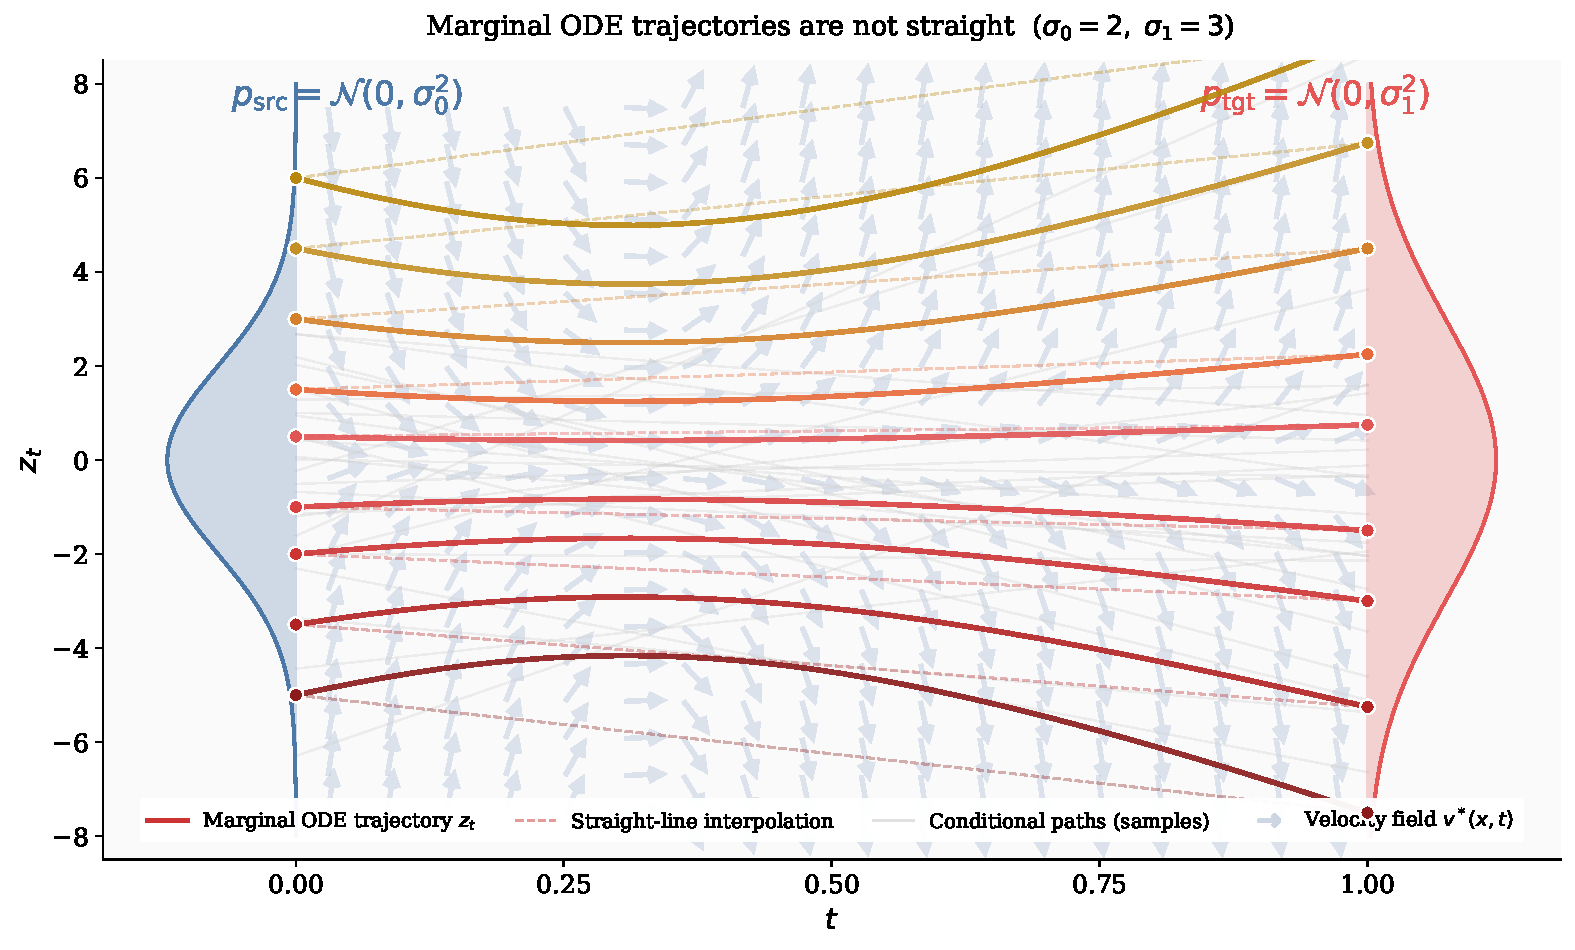
\includegraphics[width=\linewidth]{Images/PartB/straightness_counterexample.pdf}
    \caption{\textbfs{边缘 ODE 轨迹在规范仿射插值下不是直的。}
    我们将$x_0 \sim \mathcal{N}(0, \sigma_0^2)$和$x_1 \sim \mathcal{N}(0, \sigma_1^2)$与$\sigma_0=2$、$\sigma_1=3$以及独立联轴器一起使用。
    灰线显示采样条件路径 $(1-t)x_0 + tx_1$，其结构是直的。
    实线显示精确的边缘 ODE 轨迹 $z_t = z_0\sqrt{(1-t)^2 + (\sigma_1/\sigma_0)^2 t^2}$，虚线显示从 $z_0$ 到 $z_1$ 的相应直线插值。
    实线和虚线之间的可见间隙证实了 $t$ 中的边缘 ODE 轨迹不是仿射的，即使每个条件路径都是直线。
    边缘密度 $p_{\mathrm{src}}$ 和 $p_{\mathrm{tgt}}$ 分别显示在左侧和右侧边缘。
    \figcredit{由作者使用AI辅助编码创建。}}
\end{figure}
     






\clearpage
\newpage


\section{\texorpdfstring{（选读）正则仿射流的性质}{（选读）正则仿射流的性质}}\label{sec:optimal-canonical}

给定两个端点分布 $p_0=p_{\mathrm{src}}$ 和 $p_1=p_{\mathrm{tgt}}$， 
在流匹配 (FM)~\citep{lipman2022flow} 中定义条件路径的自然且广泛使用的选择 
整流流(RF)~\citep{liu2022flow}为线性插值
\[
a_t = 1 - t, \qquad b_t = t,
\]
产生插值
\[
\mathbf{x}_t = (1 - t)\mathbf{x}_0 + t \mathbf{x}_1, 
\qquad \mathbf{x}_0 \sim p_{\mathrm{src}},\ \mathbf{x}_1 \sim p_{\mathrm{tgt}}.
\]
在这种选择下，训练目标简化为
\[
\mathbb{E}_{t \sim \mathcal{U}[0,1]}   
\mathbb{E}_{\mathbf{x}_0, \mathbf{x}_1} 
\left[ \bigl\|\mathbf{v}_{\bm{\phi}}(\mathbf{x}_t, t) - (\mathbf{x}_1 - \mathbf{x}_0)\bigr\|_2^2 \right].
\]

这种线性流动具有几个吸引人的特性。 
特别是，它承认一种迭代细化方案，称为 \emph{\texttt{Reflow}}， 
它逐渐拉直分布之间的路径，同时保留边缘。 





\subsection{整流（Rectified Flow）：从嘈杂的猜测到结构化配对}\label{subsec:rectify}

\paragraph{为什么要更换联轴器？}
独立耦合下
\[
\pi(\rvx_0,\rvx_1)
=
p_{\mathrm{src}}(\rvx_0)
p_{\mathrm{tgt}}(\rvx_1),
\]
每个条件插值
$(1-t)\rvx_0+t\rvx_1$ 是一条直线。正如强调的那样
然而，\Cref{sec:optimal-canonical}，相应的边缘速度
平均来自许多不相关端点对的方向，因此诱导
边缘 ODE 轨迹不必是直线。这种弯曲的边缘动力学
仅通过几个数值步骤就很难准确积分。

纠正通过更改端点耦合来解决此问题。一个
学习到的 ODE 将每个源样本传输到模型生成的端点，
产生一个依赖耦合，随后用于定义一个新的
条件插值。

\paragraph{通过相关耦合调整流。}
我们使用预先训练的扩散模型，而不是依赖任意配对 $\rvv_{\bphi^\times}(\cdot,t)$ 作为 PF-ODE 中的漂移 \emph{确定性} 传输每个源点。开始于 $\rvz(0)=\rvz_0 \sim p_{\text{src}}$，我们整合
\[
\frac{\diff \rvz(t)}{\diff t} = \rvv_{\bphi^\times}(\rvz(t),t), \qquad t \in [0,1],
\]
获取 $\hat\rvz_1 := \rvz(1)$ 位于从预训练模型学习的数据空间附近。得到的结果对 $(\rvz_0,\hat\rvz_1)$ 形成一个 \emph{相关耦合}：它遵循结构化的模型引导路径，而不是任意插值。这个想法自然延伸到形式的仿射参考路径 $\rvx_t = a_t \rvx_0 + b_t \rvx_1$，其中 $\rvx_0 \sim p_{\text{src}}$ 和 $\rvx_1 \sim p_{\text{tgt}}$.



\begin{algorithm}[H]
\caption{\texttt{Rectify} 操作\label{alg:Rectify}}
\begin{algorithmic}[1]
\Require 参考路径 $\{\rvx_t\}_{t\in[0,1]}$ (e.g.\ $\rvx_t=a_t\rvx_0+b_t\rvx_1$)
\State \textbfs{训练前扩散。} 适合 $\rvv_{\bphi^\times}$ 在选择的路径上通过最小化
\[
\bphi^\times \in \arg\min_{\bphi} 
\mathbb{E}_{t,\rvx_0,\rvx_1} \left[\Big\|\rvv_{\bphi}(\rvx_t,t)-\frac{\diff \rvx_t}{\diff t}\Big\|_2^2\right].
\]
\State \textbfs{纠正。} 样品 $\rvz_0 \sim p_{\text{src}}$ 并集成
\[
\frac{\diff \rvz(t)}{\diff t}=\rvv_{\bphi^\times}(\rvz(t),t),\qquad \rvz(0)=\rvz_0,\quad t\in[0,1],
\]
获取 $\hat\rvz_1=\rvz(1)$ 和轨迹 $\{\rvz(t)\}_{t\in[0,1]}$.
\Ensure 相关（相干）对 $(\rvz_0,\hat\rvz_1)$ 或完整轨迹。
\end{algorithmic}
\end{algorithm}

\paragraph{为什么有效：边缘保持结构。}
让 $\bPhi_{0\to t}$ 表示由预训练扩散定义的上述 ODE 生成的流映射 $\rvv_{\bphi^\times}$;然后 $\rvz(t)=\bPhi_{0\to t}(\rvz_0)$ 和 $\hat\rvz_1=\bPhi_{0\to 1}(\rvz_0)$。的 \texttt{Rectify} 过程将每个源点与其流端点配对，给出确定性联合
\[
\pi_{\text{Rectify}}(\rvz_0,\rvz_1)
= p_{\text{src}}(\rvz_0) \delta \big(\rvz_1-\bPhi_{0\to 1}(\rvz_0)\big).
\]
我们有两个直接后果：
\begin{itemize}
    \item \textbfs{保留源边缘：} 
    $\displaystyle \int \pi_{\text{Rectify}}(\rvz_0,\rvz_1) \diff \rvz_1
    = p_{\text{src}}(\rvz_0)$.
    \item \textbfs{沿流程推进：} 
    $\displaystyle (\bPhi_{0\to t})_{\#}p_{\text{src}}=\mathrm{Law}(\rvz(t))$，即时间——$t$ 分布是推动 $p_{\text{src}}$ 通过 $\bPhi_{0\to t}$.
\end{itemize}
如果 $\rvv_{\bphi^\times}$ 匹配给定参考路径的预言机漂移 $\rvx_t$，则所有中间边缘都重合：
\[
\mathrm{Law}(\rvz(t))=\mathrm{Law}(\rvx_t),\quad \text{for all }t\in[0,1],
\quad\text{and}\quad
(\bPhi_{0\to 1})_{\#}p_{\mathrm{src}}=p_{\mathrm{tgt}}.
\]


\paragraph{摘要。}
纠正将独立端点耦合替换为学习流引起的耦合。重复下 \texttt{Reflow}，这可以产生边缘传输，并且越来越容易通过很少的数值步骤进行积分。对于规范路径，重复应用 \texttt{Rectify} (``\emph{\texttt{Reflow}}'') 在不增加运输成本的情况下进一步拉直轨迹，使训练变得更加容易。




\subsection{\texttt{Reflow}: 迭代矫直流}\label{subsec:reflow-def}

\paragraph{为什么 \texttt{Reflow}?}
独立配对通常会导致之间出现不规则且蜿蜒的 ODE 轨迹 $p_{\text{src}}$ 和 $p_{\text{tgt}}$，这会增加模拟过程中的离散化误差和方差。这就提出了一个自然的问题：

\begin{question}\label{ques:straight}
我们能否学习耦合，使传输路径更接近两个分布之间的直线，同时仍保留正确的边缘？
\end{question}

这激励 \emph{\texttt{Reflow}}: 重复申请 \texttt{Rectify} 更新耦合，以便连续流变得更容易集成。

\paragraph{核心思想：递归拉直 \texttt{Rectify}.}

从乘积耦合上的规范插值开始
$\pi^{(0)}:=p_{\text{src}}(\rvx_0)p_{\text{tgt}}(\rvx_1)$,
\[
\rvx_t=(1-t)\rvx_0+t\rvx_1.
\]
正在申请 \texttt{Rectify} 将独立配对替换为从属配对 $(\rvz_0,\hat\rvz_1)$ 由学习的 ODE 引起。重复这个过程，称为 \emph{\texttt{Reflow}}，往往会产生更直的轨迹，更容易通过少量数值步骤精确积分。精确矫直保证将在后面讨论
\Cref{subsec:reflow-properties}.

\paragraph{这 \texttt{Reflow} 程序。}
每次迭代执行两个步骤：
\begin{itemize} 
    \item \textbfs{重新安装流程：} 从当前耦合的样本训练新的速度场： \begin{align} \bm{\phi}_{k+1} &= \arg\min_{\bm{\phi}} \mathcal{L}\left(\bm{\phi}\Big\vert \pi^{(k)}\right), \quad \text{where} \notag \\ \mathcal{L}\left(\bm{\phi}\Big\vert \pi^{(k)}\right) &:= \mathbb{E}_{t, (\rvz_0^{(k)}, \hat\rvz_1^{(k)})\sim \pi^{(k)}} \left[\left\|\rvv_{\bm{\phi}}(\rvz_t, t) - (\hat\rvz_1^{(k)} - \rvz_0^{(k)})\right\|^2\right] \label{eq:reflow-loss} \end{align} 与 $\rvz_t = (1-t)\rvz_0^{(k)} + t\hat\rvz_1^{(k)}$. 
    \item \textbfs{生成新耦合：} 从新的源样本开始求解学习的 ODE $\rvz_0^{(k+1)} \sim p_{\text{src}}$: \[ \hat\rvz_1^{(k+1)} \gets \rvz_0^{(k+1)} + \int_0^1 \rvv_{\bm{\phi}_{k+1}}(\rvz(t), t) \mathrm{d}t, \] 并定义更新的耦合： \[ \pi^{(k+1)}(\rvz_0, \rvz_1) := p_{\text{src}}(\rvz_0) \delta\left(\rvz_1 - \hat\rvz_1^{(k+1)}\right). \] \end{itemize}
换句话说， \texttt{Reflow} 可以视为重复应用 \texttt{Rectify} 操作员，产生一系列逐渐细化的耦合：
\begin{align}\label{eq:rectify-op}
    \pi^{(k+1)} = \texttt{Rectify} \left(\pi^{(k)}\right)
\end{align}
使流动和耦合一起发展，产生逐渐更稳定的传输路径。



\subsection{的属性 \texttt{Reflow}}\label{subsec:reflow-properties}

两个关键的理论特性推动了 \texttt{Reflow}：它降低了运输成本并拉直了轨迹。

\paragraph{I. \texttt{Reflow} 永远不会增加运输成本。}
让 $c(\rvy)$ 是凸成本函数（例如， $\|\rvy\|_2^p$ 与 $p \geq 1$）。每个 \texttt{Rectify} 台阶形成新联轴器 $(\rvz_0, \hat\rvz_1)$ 其成本不比原来差：
\proppp{\texttt{Rectify} 可以降低运输成本}{rec-transport-cost}{
假设理想速度场 $\rvv^* = \rvv_{\bm{\phi}^\times}$，我们有：
\[
\mathbb{E}\left[c\left(\hat\rvz_1 - \rvz_0\right)\right] \leq \mathbb{E}\left[c\left(\rvx_1 - \rvx_0\right)\right].
\]
}{由 Jensen 不等式得出。参见 \citet{liu2022flow} 完整推导。}
递归应用此结果表明 \texttt{Reflow} 过程中不增加运输成本。

\paragraph{二。 \texttt{Reflow} 拉直路径。}
递归应用 \texttt{Reflow} 促进越来越直的轨迹，尽管直线度测量不能保证在每次迭代中单调改进。为了衡量这一点，定义 \emph{直线度函数} 路径的 $\mathbf{Y} = \{\rvy_t\}_{t\in[0,1]}$ 如
\[
\mathcal{S}(\mathbf{Y}) := \int_0^1 \mathbb{E}\left[\left\|\rvy_1 - \rvy_0 - \frac{\mathrm{d}\rvy_t}{\mathrm{d}t} \right\|_2^2 \right]  \mathrm{d}t.
\]
如果 $\mathcal{S}(\mathbf{Y}) = 0$，那么 $\mathbf{Y}$ 正好是一条直线。

\proppp{\texttt{Reflow} 拉直随机路径}{reflow-straight}{
用于修正路径 $\rmZ^{(k)}$，我们有：
\[
\min_{k \in \{0,\dots,K\}} \mathcal{S}(\rmZ^{(k)}) \leq \frac{\mathbb{E}\left[\|\rvx_1 - \rvx_0\|^2\right]}{K}.
\]
}{参见定理 3.7 \citet{liu2022flow}.}

\begin{figure}[t]
    \centering
    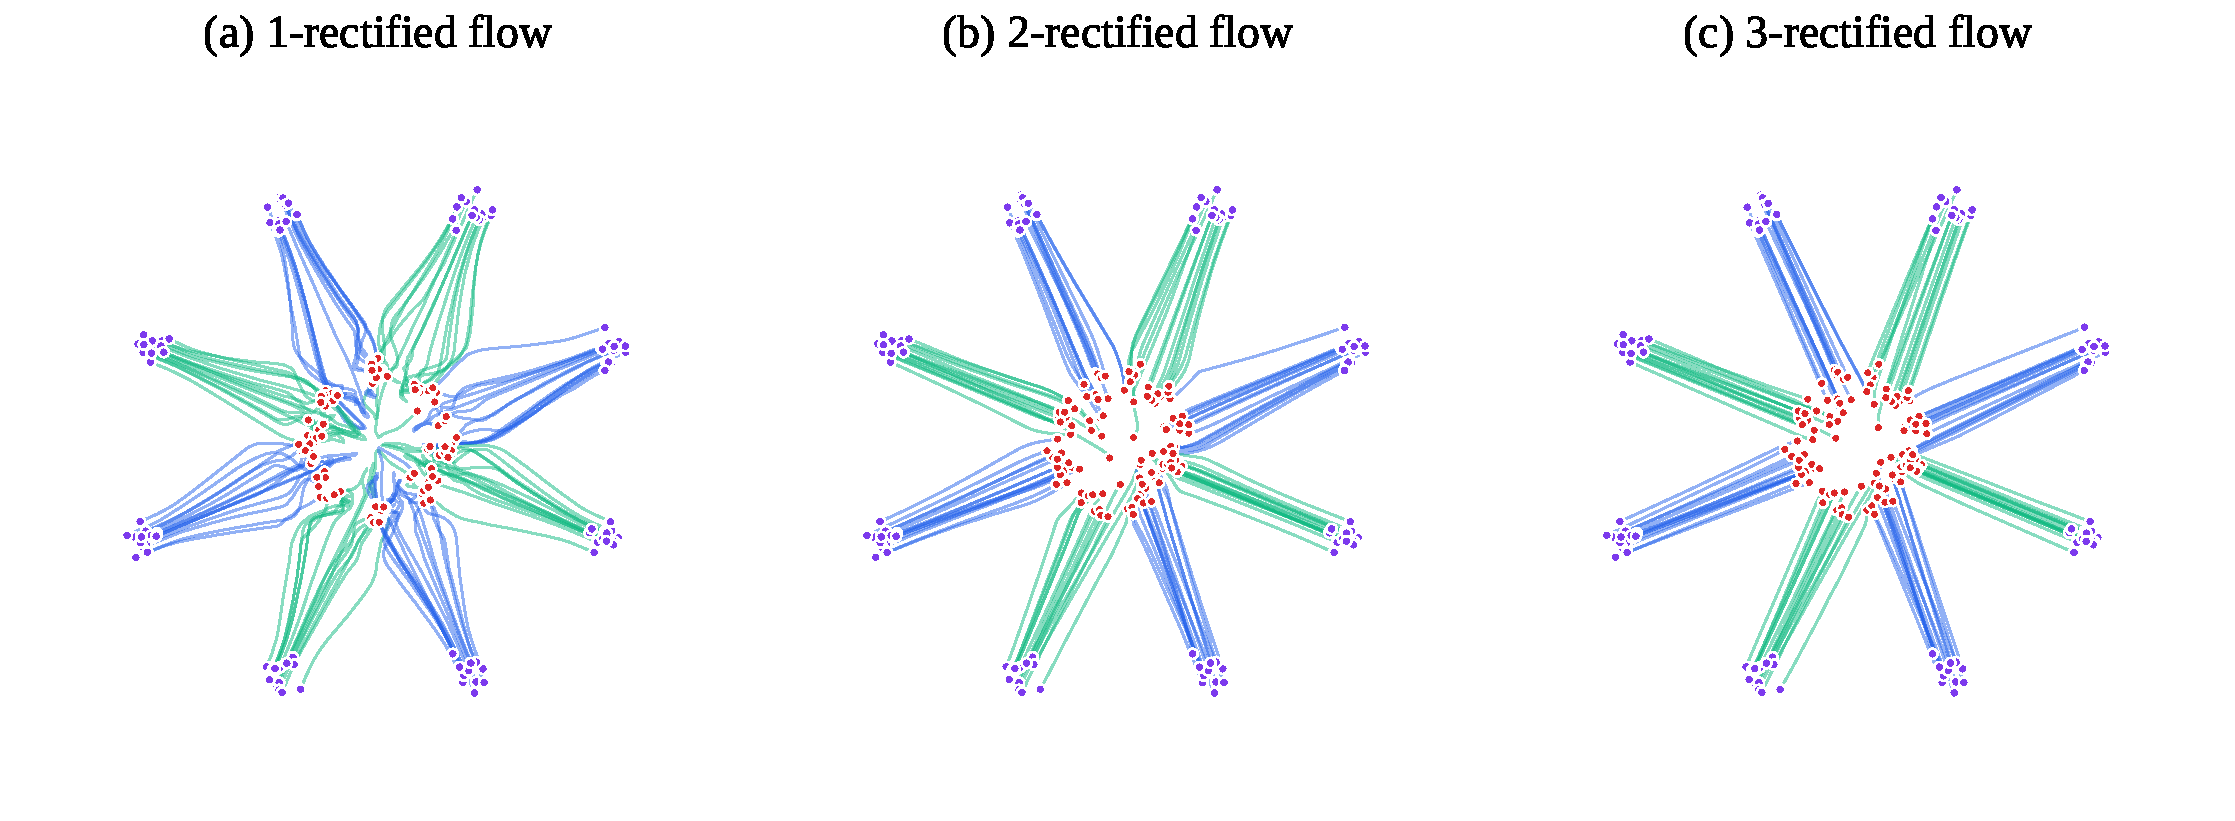
\includegraphics[width=\textwidth]{Images/PartB/rectified_flow_trained.pdf}
    \caption{\textbfs{插图 \texttt{Reflow}.} 路径逐渐变得直 \texttt{Rectify} 程序。  \figcredit{改编自 \citet{liu2022flow}.}}
    \label{fig:ill_Reflow}
\end{figure}


具有线性插值内核的 FM 或 RF 公式，以及 \texttt{Reflow} 程序，提供了更简单的训练目标和细化随机耦合的实用方法。有关理论详细信息，我们建议读者参考 \citep{liu2022flow, liu2022rectified}.



\paragraph{三．连接到最优传输。}
最后，我们注意到直线耦合在最优传输（OT）意义上不一定是最佳的。这涉及到一些术语，稍后会介绍 \Cref{sec:ot-intro};因此，我们建议不熟悉旧约的读者阅读该部分。二次成本最优传输的一个标志是粒子沿直线运动：粒子在 $\rvx_0$ 移至 $\rmT(\rvx_0)$ 通过 $\rvx_t = (1 - t)\rvx_0 + t \rmT(\rvx_0)$，其中 $\rmT$ 是最优传输图。然而，并不是每张映射 $\rmS$ 生成这样的直线路径，即 $\rvx_t = (1 - t)\rvx_0 + t \rmS(\rvx_0)$，是最佳的。映射 $\rmS$ 仅当 Monge 成本最小化时才产生最佳流 $\mathbb{E}[\|\rvx_0 - \rmS(\rvx_0)\|^2]$。因此，虽然直线路径是必要的，但它们还不够。最优性还取决于正确的端点图 $\rmT$.

\exm{直联轴器不一定是最佳的}{
让 $p_{\text{src}} = p_{\text{tgt}} = \mathcal{N}(\bm{0}, \rmI)$。为了成本 $c(\rvx, \rvy) = \|\rvx - \rvy\|^p$ 与 $p > 0$， $c$-最佳耦合是恒等耦合 $\pi^{*}$，其中 $\pi^{*}$ 是定律 $(\rvx, \rvx)$ 与 $\rvx \sim p_{\text{src}}$。现在考虑耦合 $\pi_{\rmA}$ 定义为定律 $(\rvx, \rmA \rvx)$，其中 $\rvx \sim p_{\text{src}}$ 和 $\rmA$ 是满足的旋转矩阵 $\rmA^\top \rmA = \rmI$, $\det(\rmA) = 1$, $\rmA \neq \rmI$, 和 $-1$ 不是特征值。然后 $\pi_{\rmA}$ 是有效的耦合 $p_{\text{src}}$ 和 $p_{\text{tgt}}$，并且对应于之间的直线路径 $\rvx$ 和 $\rmA \rvx$，但事实并非如此 $c$-对于任何二次可微的严格凸成本来说是最佳的 $c$ 具有可逆 Hessian 矩阵。次优性是由旋转变换引起的。正如中所讨论的 \Cref{eq:reflow-loss-gradient}，即使移除旋转也可能不会导致最佳耦合。
}

我们将继续探索与 OT 的联系 \Cref{subsec:ot-linear-reflow}.

\clearpage
\newpage

\newpage
\section{结束语}\label{sec:ch5_cr}
     
本章阐明了扩散模型的第三个也是最后一个基本观点，该观点植根于确定性流的原理。我们的探索从归一化流（NF）开始，它利用变量替换公式来学习简单先验和数据分布之间的精确可逆映射。然后，我们看到这个概念演变为神经常微分方程的连续时间过程，其中学习的速度场控制着转换。然而，这种方法有一个显着的缺点，即需要在训练循环中进行昂贵的 ODE 模拟。



现代流匹配 (FM) 框架是应对这一挑战的优雅而高效的解决方案。通过预先定义概率路径$\{p_{t}\}_t$和满足连续性方程的相应速度场，FM为ODE流建立了明确的目标。至关重要的是，正如我们在变分和基于分数的视图中看到的那样，FM 采用了强大的调节技巧。这将边缘速度场匹配的棘手问题转化为针对已知条件速度的简单且易于处理的回归，从而使训练完全无需模拟。这种观点将扩散模型本身重塑为学习确定性流以在数据分布之前传输高斯分布的特殊情况。




随着基于流的视图的引入，我们对扩散建模的三个概念支柱的调查现已完成。在整个旅程中，出现了一个显着的模式：每个框架尽管起源于 VAE、EBM 或 NF，但都收敛于连续时间生成过程，并依赖调节策略来实现易于处理的学习。

在下一章中，我们最终将把这些并行线程综合到一个统一的框架中。我们将：
\begin{enumerate}
    \item 正式证明变分、基于分数和基于流程的观点不仅相似，而且在基本层面上在数学上是等效的。
    \item 展示福克-普朗克方程如何作为控制所有三种视图中密度演化的普遍法则，揭示它们只是描述相同核心生成原理的不同镜头。
\end{enumerate}

这个统一的视角将提供对现代扩散范式的完整和系统的理解。